%!TEX root=../main.tex

{
\setstretch{1.2}

\section*{Аннотация}

% \vspace{-0.5cm}
Алгоритмы планирования задач на вычислительных кластерах являются предметом активных исследований. Проведение таких исследований на настоящем кластере долго и дорого, поэтому для сравнения различных гипотез используются симуляторы. Качество получаемых результатов во многом зависит от точности используемой модели. Большинство современных симуляторов используют простые модели, которых не всегда достаточно. Эта работа сосредоточена на разработке симулятора вычислительного кластера на базе фреймворка \texttt{DSLab}, который позволяет очень точно и гибко моделировать сценарии вычислительной нагрузки с использованием примитивов асинхронного программирования. \texttt{DSLab} предоставляет массу возможностей как для написания новых алгоритмов, так и для использования готовых модулей различных компонент распределенной системы. Разработанный симулятор получил основные преимущества \texttt{DSLab} и позволяет моделировать работу алгоритмов упаковки заданий на кластер и алгоритмов справедливого распределение ресурсов.

% \vspace{-0.5cm}
\section*{Ключевые слова}

Распределенные системы, вычислительный кластер, алгоритмы планирования, управление ресурсами, имитационное моделирование, симулятор

% \vspace{-0.5cm}
\section*{Annotation}
% \vspace{-0.5cm}
Algorithms for scheduling tasks on compute clusters are the subject of active research. It is quite expensive to conduct such studies using real cluster, so simulators are used to compare different hypotheses. The quality of the results obtained largely depends on the accuracy of the model used. Most modern simulators use simple compute models, which are not always enough. Our work is focused on developing a simulator of a compute cluster based on the \texttt{DSLab} framework, which will allow very accurate and flexible modeling of computational load scenarios using asynchronous programming primitives. \texttt{DSLab} provides a lot of opportunities both for writing new algorithms and using ready-made modules of various distributed system components. Thus, the new simulator has received the main advantages of \texttt{DSLab} and allows modeling resource packaging algorithms and fair resource sharing algorithms in complex configurations.


% \vspace{-0.5cm}
\section*{Keywords}
Distributed systems, compute cluster, scheduling algorithms, resource management, imitational modeling, simulator

}

\newpage 

\section{Введение}

Вычислительные кластеры, состоящие из набора серверов с различными ресурсами (процессор, память, диск), широко применяются для проведения сложных расчетов и обработки больших объемов данных в науке и бизнесе. На большом промышленном кластере одновременно могут выполняться тысячи заданий (batch jobs) различных пользователей, а часть заданий может находиться в очереди в ожидании выделения ресурсов. Запуском заданий и распределением ресурсов между ними управляет менеджер кластера или планировщик. В основе работы менеджера кластера лежат алгоритмы планирования задания (job scheduling), основной целью которых является максимально эффективное использование ресурсов кластера. Данные алгоритмы являются предметом активных исследований. Проводить такие исследования на реальном кластере долго и дорого, поэтому необходима компьютерная модель (симулятор), позволяющая быстро проверить гипотезу или провести сравнительное тестирование разных алгоритмов на некоторой истории нагрузки кластера. Подобный симулятор также может использоваться в учебном процессе для знакомства студентов с такими системами и возникающими в них задачами.

\subsection{Актуальность и значимость}

Алгоритм планирования заданий -- ключевая часть архитектуры всех вычислительных кластеров. Поиск оптимальных алгоритмов очень актуален, поскольку повышение утилизации имеющихся ресурсов позволит существенно снизить затраты на оборудование кластера и ускорить его работу. Существующие симуляторы в основном предлагают простые модели задач или углубляются в конкретную область (например, глубинное обучение). 

Новый симулятор, разработанный на базе фреймворка \texttt{DSLab} позволит исследователям подбирать алгоритмы под конкретные сценарии нагрузки, используемые в их кластере. Таким образом, симулятор позволит более точно предсказывать поведение настоящего кластера.  

\subsection{Цели и задачи ВКР}

Целью ВКР является разработка симулятора вычислительного кластера на базе фреймворка \texttt{DSLab}. 

Для достижения этой цели были поставлены следующие задачи: 
\begin{enumerate}
\item  Изучить литературу по теме и существующие симуляторы, подготовить обзор с анализом их преимуществ и недостатков.
\item Поэтапно реализовать компоненты симулятора, покрыть их тестами и снабдить комментариями.
\item Подготовить и провести эксперименты, демонстрирующие работоспособность симулятора и достижение всех требований.
\item Подготовить документацию пользователя.
\end{enumerate}

\subsection{Основные результаты работы}

В результате ВКР был разработан эффективный и многофункциональный симулятор вычислительного кластера на базе фреймворка \texttt{DSLab}, были реализованны несколько популярных алгоритмов планирования задач и проведены тесты на данных трейсов различных компаний, а также синтетических данных. 


\subsection{Структура работы}

Дальнейшая структура работы следующая: 
\begin{itemize}
    \item Глава \ref{sec:lit-review} содержит обзор литературы и существующих симуляторов.
    \item Глава \ref{sec:dslab} описывает фреймворк \texttt{DSLab} и его асинхронное расширение, на базе которого был разработан симулятор.
    \item Глава \ref{sec:main-impl} описывает реализацию симулятора, основные компоненты и используемые модели.
    \item Глава \ref{sec:experiments} содержит описание проведенных экспериментов на разработанном симуляторе и их анализ.
    \item Глава \ref{sec:conclusion} подводит итоги работы и предлагает дальнейшие направления разработки и улучшения симулятора.
\end{itemize} 

\section{Обзор литературы}\label{sec:lit-review}


\subsection{Вычислительная модель в симуляции}

Для моделирования работы кластера и алгоритмов планирования требуется модель рабочей нагрузки. Самая распространенная модель описывает рабочую нагрузку как набор заданий (jobs), состоящих из задач (tasks), которые непосредственно исполняются на кластере и потребляют ресурсы. Структура этих заданий может быть нескольких видов: 
\begin{itemize}
  \item Фиксированное задание (rigid job) -- заранее известны требования к ресурсам задания.
  \item Масштабируемое задание (moldable job) -- существует набор конфигураций ресурсов, на которых можно запустить задание. Конфигурация выбирается на этапе планирования и не изменяется по ходу исполнения. 
  \item Гибкое задание (malleable job) -- задание, которое может адаптивно менять количество используемых ресурсов в процессе выполнения.
\end{itemize}

Требования к планированию заданий делятся на две категории:
\begin{itemize}
  \item Раздельное планирование. Задачи (составные части задания) могут планироваться на кластере по мере освобождения ресурсов, при этом между ними могут быть зависимости. Самый распространенный пример такой модели планирования -- концепция MapReduce\cite{mapreduce-article}.
  \item Комплектное планирование (gang scheduling). В такой модели задание воспринимается как параллельная программа, все задачи которой нужно одновременно запустить.
\end{itemize}

Среди распространенных форматов описания нагрузки на кластер можно выделить Standard Workload Format(SWF)\cite{standard-workload-format}. Этот формат широко используется в литературе и поддерживается многими симуляторами. Однако, SWF предоставляет довольно мало информации о рабочей нагрузке. Ключевая информация задании включает время прибытия, время выполнения, приоритет и потребность в ресурсах. Единственное предположение, которое мы можем сделать о рабочей нагрузке заключается в том, что задание потребляет все выделенные ресурсы во время выполнения. Наиболее популярные трейсы рабочей нагрузки представлены в аналогичном формате (например, Google trace\cite{google-clusterdata}).

Однако, существует и более сложный подход к моделированию задач на кластере, при котором время выполнения задачи рассчитывается на основе структуры рабочей нагрузки и доступных ресурсов. Основное преимущество этого подхода заключается в том, что больше деталей задачи могут быть учтены и использованы при планировании. Кроме того, появляется возможность с большей точностью рассчитать загрузку кластера и поведение его компонент. Основной недостаток -- для такого моделирования довольно сложно найти данные из открытых источников, поскольку информация о детальной структуре задач обычно конфиденциальна и не публикуется.

\subsection{Аналоги} 

Существующие симуляторы относятся к одной из двух категорий: симуляторы, созданные с нуля, и основанные на готовой платформе. Другой способ группировки симуляторов -- по типу рабочей нагрузки, которую они поддерживают: симуляторы, которые работают с SWF или аналогичными форматами, и поддерживающие сложное описание рабочей нагрузки.

\subsubsection{AccaSim}

Характерным примером такого симулятора <<с нуля>> является \texttt{AccaSim}\cite{accasim-article}. Он основан на дискретно-событийном моделировании и содержит предопределенные алгоритмы планирования. Он довольно прост в использовании, но не поддерживает сложные конфигурации. На вход принимаются только файлы в формате SWF. В отличие от \texttt{AccaSim}, наш симулятор сможет моделировать произвольные сценарии рабочей нагрузки, которые будут определены пользователями. Кроме того, наш симулятор является модульным, поскольку основан на \texttt{DSLab}. Пользователи смогут подключать модули, написанные другими исследователями в рамках платформы \texttt{DSLab}, и использовать их в своих экспериментах. Например, \texttt{DSLab} предоставляет модели сети, которые могут точно симулировать различные топологии. Среди преимуществ этого симулятора можно отметить, что он поддерживает инкрементальное чтение трейса нагрузки, что делает возможным проведение больших симуляций.

\subsubsection{BatSim}

Симулятор \texttt{BatSim} основан на \texttt{SimGrid}\cite{simgrid-article} и позволяет разработчикам интегрировать алгоритмы на нескольких языках на основе inter-process communication. Подробное сравнение \texttt{SimGrid} и \texttt{DSLab} можно найти в документации по \texttt{DSLab}\cite{dslab-analog-cmp}. Ключевое ограничение \texttt{BatSim} -- из возможных ресурсов кластера он поддерживает моделирование только <<вычисления>>, <<передачи данных>> и <<операции с распределенной файловой системой>>. \texttt{BatSim} предоставляет интерфейс для настройки пользовательских типов рабочей нагрузки, но они ограничены несколькими заданными паттернами и возможными последовательными комбинациями из них (см. рис. \ref{fig:batsim-profile}). 

\begin{figure}[h]
    \footnotesize  
\begin{jsoncode}
"jobs": [
  {"id":"simple", "subtime":1, "res": 4, "profile": "simple"},
],
"profiles": {
  /* workload profile definition */
  "simple": {
    "type": "parallel",
    "cpu": [5e6,  0,  0,  0],
    "com": [5e6,  0,  0,  0,
            5e6,5e6,  0,  0,
            5e6,5e6,  0,  0,
            5e6,5e6,5e6,  0]
  },
}
\end{jsoncode}
\caption{Пример описания нагрузки в \texttt{BatSim}}
\label{fig:batsim-profile}
\end{figure}

Также из рис. \ref{fig:batsim-profile} можно увидеть, что потребность в ресурсах задачи выражается в количестве выделенных <<ресурсов>> (одно число -- количество серверов), и задача размещается на них целиком. Таким образом, существенно ограничивается моделирование задач с разным профилем требований к ресурсам (задача упаковки). Стоит отметить, что каждый сервер имеет свою вычислительную мощность, а также каким-то образом размещен в топологии сети, поэтому проблема размещения задач оптимальным образом на кластере не сводится к тривиальной. Необходимость учитывать топологию сети в такой модели -- сложная проблема планирования. Однако, проблема упаковки задач на несколько ресурсов в такой модели не рассматривается.

Наш симулятор расширит подход \texttt{BatSim} для определения произвольной рабочей нагрузки, но при этом предоставит больше возможностей для управления ресурсами (процессор, память, диск), а также предоставит еще больше возможностей для описания сценария нагрузки с использованием примитивов асинхронного программирования.

\subsubsection{IRMaSim}

Дальнейшим развитием \texttt{BatSim} стал симулятор \texttt{IRMaSim}\cite{irmasim-article}. В нем отмечаются недостатки \texttt{BatSim} в точности моделирования вычислений и предоставляются намного более точные модели процессоров и добавляются различные модели оперативной памяти. В этом симуляторе возможно точно указать тип оперативной памяти и ее скорость, и все это будет учитываться в симуляции. Также этот симулятор поддерживает сценарии работы с задачами глубинного обучения (Deep Reinforcement Learning). Однако, ключевое ограничение остается то же -- потребность задач в ресурсах указывается одним числом -- количеством <<ресурсов>> (серверов). По аналогии с \texttt{BatSim}, этот симулятор фокусируется на потреблении энергии в процессе работы кластера и позволяет разрабатывать алгоритмы планирования, оптимизирующие энергопотребление. 

\subsubsection{ElastiSim}

Симулятор \texttt{ElastiSim}\cite{elastisim-article} также основан на \texttt{SimGrid} и ориентирован на гибкие рабочие нагрузки (malleable workloads). Это позволяет моделировать динамические изменения количества ресурсов, выделяемых на исполнение задач. Одна из важных особенностей \texttt{ElastiSim} -- высокая точность моделирования задач глубинного обучения, для которых он и предназначен. Кроме этого, в \texttt{ElastiSim} поддерживается моделирование передачи данных (I/O) по сети. Авторы обращают особое внимание на то, что операции I/O могут стать узким местом, поскольку объем передаваемых данных постоянно увеличивается. Выполнение каждой задачи состоит из нескольких этапов и может быть настроено с помощью файла JSON путем объединения предварительно определенного набора операций: CPU, GPU, операций I/O и дисковых операций. Это самый продвинутый симулятор из всех рассмотренных источников. Мы будем стремиться предоставить еще больше возможностей для подробного описания выполняемых задач, однако наш симулятор будет поддерживать более распространенную модель вычислений, при которой каждой задаче выделяется фиксированная аллокация ресурсов на время выполнения.

\subsection{Выводы}

Рассмотренные симуляторы решают разные задачи симуляции: симуляция упаковки задач на кластер в условиях нескольких ресурсов (\texttt{AccaSim}), и точная симуляция вычислительного процесса (\texttt{BatSim}, \texttt{IRMaSim}, \texttt{ElastiSim}). При этом ни в одном симуляторе эти задачи не пересекаются. Наш симулятор разработан в более общей модели, что позволяет поддержать задачу упаковки и точное моделирование вычислений одновременно. Более того, одной из тем исследований планирования задач на кластерах является справедливость (в условиях, когда кластер делится между несколькими пользователями). Задача справедливости распределения ресурсов не рассматривалась в приведенных симуляторах, однако наш симулятор поддерживает и эту возможность. Наглядное сравнение симуляторов можно увидеть в таблице \ref{tab:sim-compare}. Разработанный симулятор называется \texttt{DSLab-CS} (\texttt{DSLab} Cluster Simulator).

\begin{table}[h!]
  \small
\centering
\begin{tabular}{|c|c|c|c|c|c|}
\hline
\textbf{Критерий} & \texttt{DSLab-CS} & \texttt{AccaSim} & \texttt{BatSim} & \texttt{IRMaSim} & \texttt{ElastiSim} \\
\hline
Платформа симулятора & \texttt{DSLab} & \texttt{Custom} & \texttt{SimGrid} & \texttt{SimGrid} & \texttt{SimGrid} \\
\hline
Язык программирования & \texttt{Rust} & \texttt{Python} & \texttt{C++} &  \texttt{C++} &  \texttt{C++} \\
\hline
\makecell{Поддержка других языков \\ программирования для \\ алгоритмов пользователей} & -- & -- & + & + & + \\
\hline
Форматы заданий & rigid & rigid & rigid & rigid & \makecell[cc]{rigid\\moldable\\malleable} \\
\hline
Поддержка форматов трейсов & \makecell[cc] {
  SWF\\
  Custom\\
  Alibaba trace\\
  Google trace
} & SWF & \makecell[cc]{SWF\\Custom} & \makecell[cc]{SWF\\Custom} & Custom \\
\hline 
\makecell[cc]{
  Поддержка итеративного \\ чтения трейса нагрузки \\ для длительных симуляций
} & + & + & -- & -- & -- \\
\hline 
\makecell[cc]{
Поддержка сложных \\ моделей сети} & + & -- & + & + & + \\
\hline
\makecell[cc] {
  Поддержка разных моделей \\ оперативной памяти
} & -- & -- & -- & + & -- \\
\hline 
\makecell[cc] {
  Поддержка модели GPU и \\ операций глубинного обучения
} & -- & -- & -- & + & + \\
\hline
\makecell[cc]{
  Поддержка моделирования \\ упаковки задач на кластер \\ c несколькими ресурсами 
} & + & + & -- & -- & -- \\
\hline
\makecell[cc]{
  Поддержка моделирования \\ упаковки задач на кластер \\ с учетом топологии сети
} & + & -- & + & + & + \\
\hline 
\makecell[cc]{
  Поддержка моделирования \\ справедливого распределения \\ ресурсов между пользователями
} & + & -- & -- & -- & -- \\
\hline
\makecell[cc]{
Поддержка описания \\ сложных профилей нагрузки \\ через файлы конфигурации }& + & -- & + & + & + \\
\hline  
\end{tabular}
\caption{Сравнение симуляторов}
\label{tab:sim-compare}
\end{table}



\section{Фреймворк DSLab}\label{sec:dslab}

\subsection{Архитектура DSLab}


В качестве платформы для реализации симулятора выбран \texttt{DSLab} -- модульный фреймворк для моделирования и тестирования распределенных систем. Модули можно разделить на 3 группы: базовые, универсальные и специализированные (см рисунок \ref{fig:dslab_arc}). За основу взят подход дискретно-событийного моделирования, при котором компоненты симуляции обмениваются событиями через базовый низкоуровневый модуль \texttt{dslab-core}. Соответственно, пользовательская логика каждого компонента состоит из обработки входящих событий от других компонент и отправки новых. Универсальные модули могут использовать исследователями соответствующих предметных областей, например, разработанный симулятор вычислительного кластера использует готовые модули вычислений, сети и диска (подробнее об этом в главе \ref{cluster-model}). 

\begin{figure}[H]
    \centering
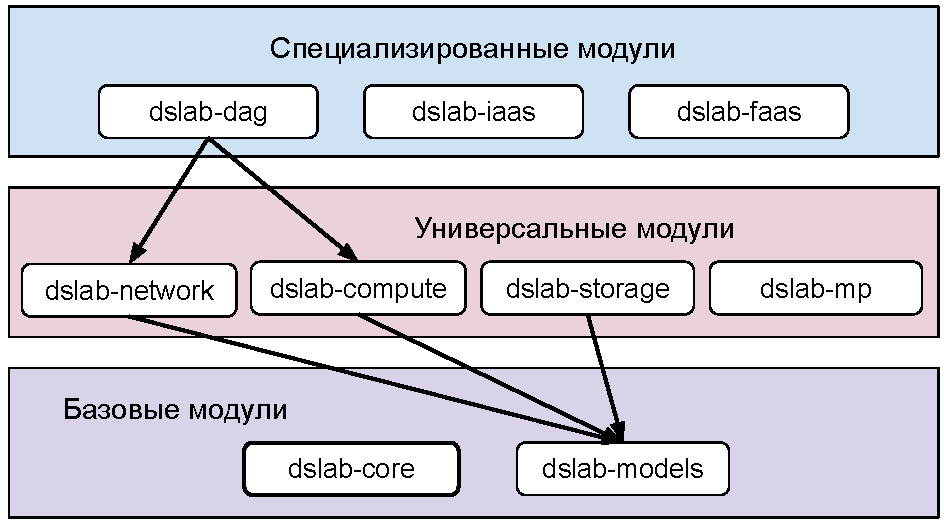
\includegraphics[width=0.7\linewidth]{images/dslab_arc}
\caption{Архитектура \texttt{DSLab}}
\label{fig:dslab_arc}
\end{figure}

Описание архитектуры основано на официальной документации \cite{dslab-architecture}. Реализация всех модулей опубликована в GitHub-репозитории\cite{dslab-repo}. Полное сравнение с другими симуляторами можно также найти в документации\cite{dslab-analog-cmp}.

\subsection{Асинхронное управление событиями}

В предыдущей работе была добавлена возможность управлять событиями \texttt{DSLab} асинхронно\cite{async-dslab}, что существенно расширило возможности написания компонент и сделало возможным ключевую особенность нового симулятора -- описание профиля нагрузки задач через асинхронные примитивы языка \texttt{Rust} (подробнее об этом в главе \ref{compute-model}). Ключевая особенность такого расширения -- возможность спрятать от пользователя явную работу с событиями, предоставив ему высокоуровневые асинхронные функции, в реализации которых зашито асинхронное ожидание внутренних событий. Например, при работе с записью на диск можно предоставить пользователю асинхронную функцию (см рисунок \ref{fig:async-write}). 
\begin{figure}[h]
    \footnotesize
    \begin{rustcode}
pub async fn write_data(&self, size: u64) -> Result<(), String> {
  let req_id = self.disk.write(size, /*requester=*/self.ctx.id());

  select! {
    _ = self.ctx.recv_event_by_key::<DataWriteCompleted>(req_id).fuse() => {
        Result::Ok(())
    }
    failed = self.ctx.recv_event_by_key::<DataWriteFailed>(req_id).fuse() => {
        Result::Err(failed.data.error)
    }
  }
}
    \end{rustcode}
    \caption{Пример асинхронной функции записи данных на диск.}
    \label{fig:async-write}
\end{figure}

В этом примере используется ожидание события по ключу: исполнение функции прерывается до того момента, пока компонент (в данном случае -- вычислительный сервер, на котором запущена задача) не получит событие от собственного диска о том, что запись завершилась (либо успешно, либо с ошибкой -- для альтернативного ожидания используется макрос \texttt{select!} из библиотеки \texttt{futures}\cite{rust-futures}), после этого ядро симуляции продолжит исполнение и результат вернется пользователю.  

Таким образом, пользователю не нужно будет самостоятельно следить за событиями компонент и можно будет разделить инструкции выполнения задач от конкретных компонент, предоставив лишь <<сценарий работы>> в виде асинхронных функций. 

Точно таким же образом реализованы и другие примитивы: вычисления и  работа с сетью. 


\section{Реализация симулятора}\label{sec:main-impl}


\subsection{Архитектура симулятора}

По аналогии с самим фреймворком \texttt{DSLab} симулятор модульный, его архитектура представлена на рисунке \ref{fig:arch}.

\begin{figure}[h!]
    \centering 
    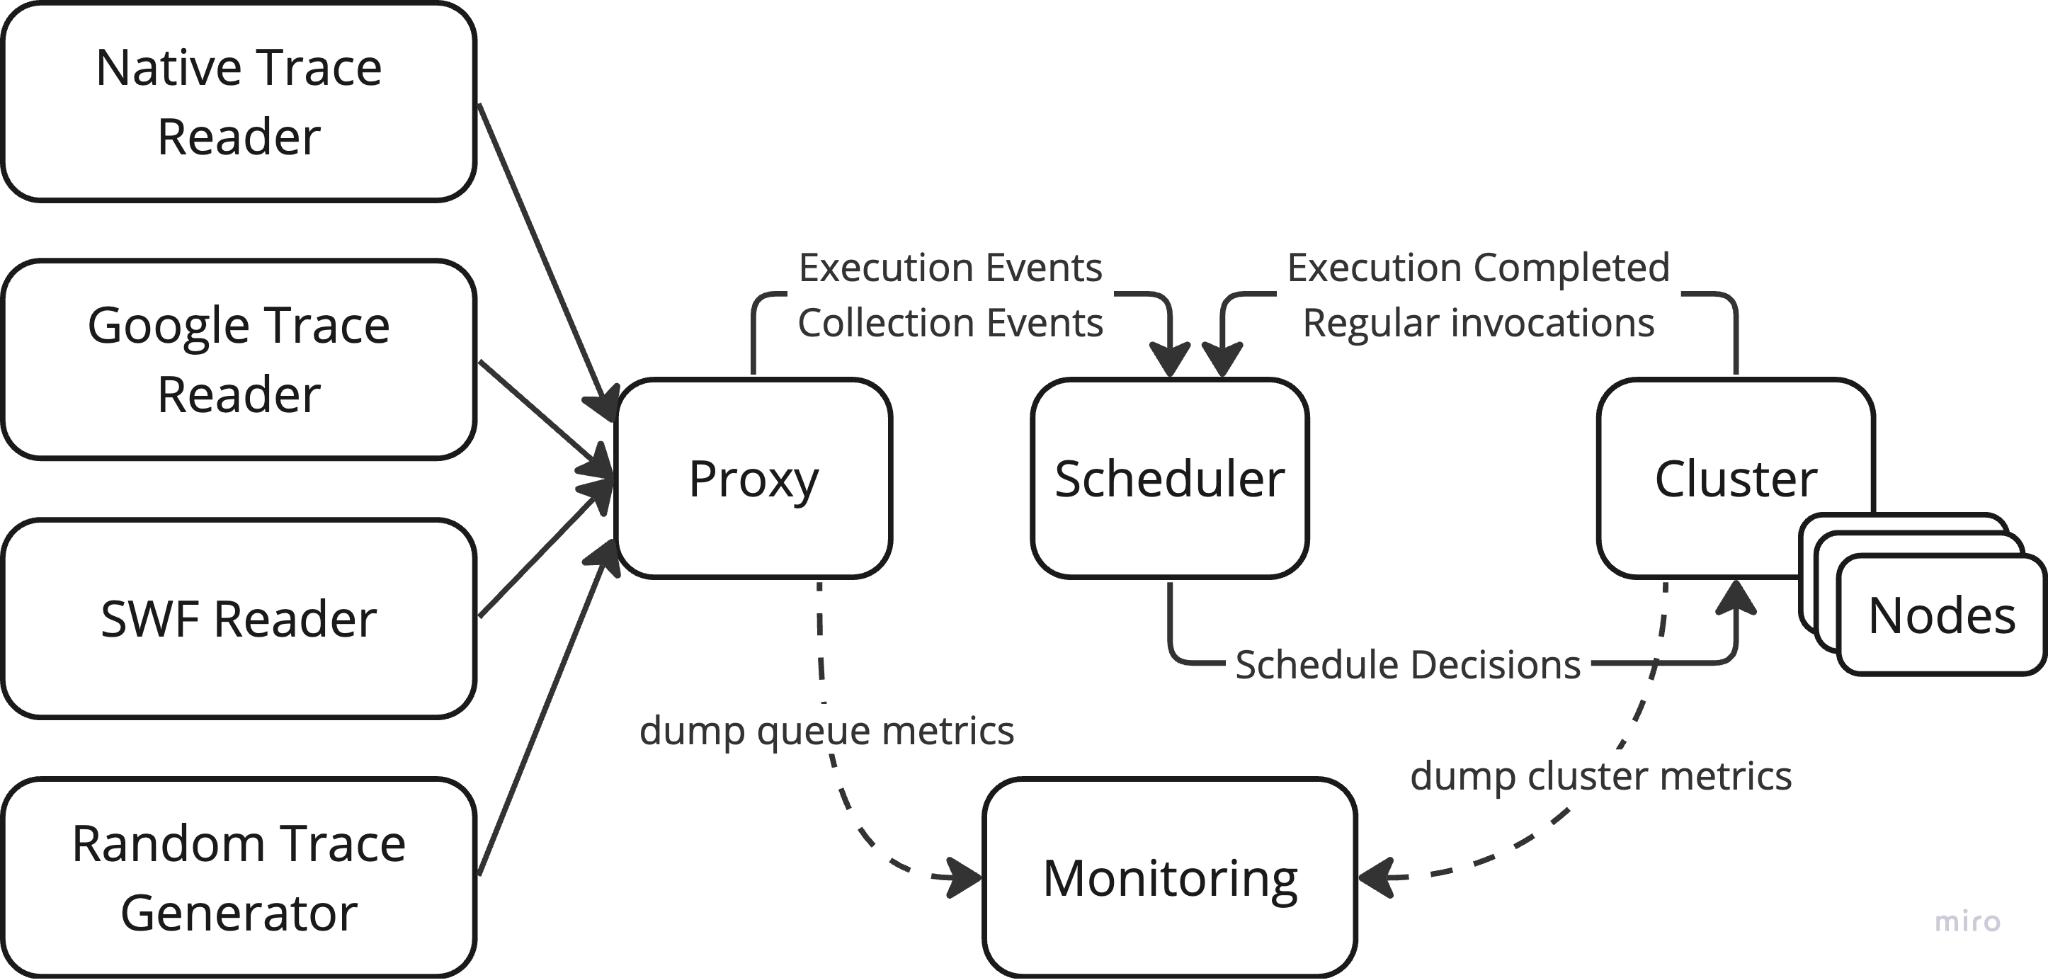
\includegraphics[width=\textwidth]{images/simulator_arc}
    \caption{Архитектура симулятора}
    \label{fig:arch}
\end{figure}

Симулятор может работать в нескольких режимах, принимая на вход несколько видов входных данных. Это может быть как готовый трейс нагрузки из открытых источников (например, Google Trace), так и пользовательский ввод задач, описанный в виде \texttt{YAML}-файла (подробнее в разделе \ref{sec:input-format-trace}).

Собирая информацию с компонентов \texttt{Proxy} и \texttt{Cluster} можно получить статистику о работе кластера и алгоритмов планирования. Например, насколько загружен кластер, насколько хорошо утилизируются его ресурсы. Такие выходные данные могут быть использованы для анализа работы алгоритмов и сравнения их эффективности. За это отвечает отдельный компонент -- \texttt{Monitoring}(подробнее в разделе \ref{sec:output-monitoring}).


\subsection{Модель кластера}\label{cluster-model}
Вычислительный кластер -- это набор отдельных серверов, которые могут быть связаны между собой моделируемой сетью (подробнее в разделе \ref{sec:network-model}). 
В симуляторе используются готовые модули \texttt{DSLab}, из которых собирается каждый сервер (см. таблицу \ref{tab:server_modules}). 
\begin{table}[h]
    \centering
    \begin{tabular}{|l|l|c|}
    \hline
    \textbf{Название модуля} & \textbf{Используемый модуль} & \textbf{Обязательный} \\
    \hline
    \texttt{compute} & \texttt{dslab\_compute::multicore::Compute} & да \\
    \hline
    \texttt{network} & \texttt{dslab\_network::Network} & нет  \\
    \hline
    \texttt{disk} & \texttt{dslab\_storage::disk::Disk} & нет \\
    \hline
    \end{tabular}
    \caption{Модули каждого сервера в кластере}
    \label{tab:server_modules}
\end{table}

Все эти модули конфигурируются при создании кластера. В случае, если хост запланировано выходит из строя или начинает работу после начала симуляции, его модули все равно создаются сразу как компоненты симуляции \texttt{DSLab}. Это необходимо, поскольку каждый сервер и каждый модуль сервера является обработчиком событий в симуляции и должен быть соответствующим образом зарегистрирован.

\subsubsection{Модуль вычислений}

Для вычислений используется модуль \texttt{Compute} с фиксированными слотами -- <<аллокациями>>, которые состоят из некоторого количества ядер процессора и объема выделенной оперативной памяти. В текущей используемой модели аллокации не могут пересекаться, однако могут быть заняты не полностью, что скажется на утилизации кластера. Т.е. на данном этапе планировщик не имеет возможность выделить больше ресурсов чем есть на сервере в надежде, что запущенные задачи используют меньше, чем просят. 

Поскольку некоторые трейсы нагрузки не содержат точную информацию о конфигурации кластера, единицы измерения <<ядер процессора>> и размера оперативной памяти могут быть относительны. Например, в Google Trace\cite{google-clusterdata} размер оперативной памяти и количества ядер процессора указаны как доля от максимального значения в кластере. Аналогичным образом нормированы и требования задач к ресурсам. Такой политики компании придерживаются с целью не раскрывать реальные конфигурации своих серверов и требования к задачам. Поскольку модуль \texttt{Compute} принимает на вход целые числа (количество ядер и объем памяти), то при создании кластера в симуляции данные в трейсе доли умножаются на большие константы таким образом, чтобы получились целые числа и погрешность была небольшой (очевидно, что при этом теряются единицы измерения). Все константы задаются пользователем при конфигурации симуляции. 

Подробнее описание модуля \texttt{Compute} и примеры использования можно посмотреть в официальной документации \texttt{DSLab}\cite{dslab-compute-docs}.

\subsubsection{Модуль сети}\label{sec:network-model}

Модуль сети \texttt{Network} содержит несколько моделей на выбор, которыми можно воспользоваться в симуляции:
\begin{enumerate}
    \item \texttt{ConstantBandwidthNetworkModel} -- самая простая модель, которая предполагает, что все сервера в кластере соединены сетью с постоянной пропускной способностью. Нагрузка сети одними компонентами никак не влияет на другие. Подходит для простой и быстрой симуляции сетевого взаимодействия с потерей в точности.
    \item \texttt{SharedBandwidthNetworkModel} -- модель, предполагающая наличие одного сетевого канала, общего для всех участников сети. Может быть достаточно точной в ситуации, когда все компоненты сети подключены к одному центральному коммутатору и пропускная способность сети много превосходит пропускную способность центрального коммутатора, являющегося узким местом. Однако, в реальности для такого случая можно применить модель \texttt{Star-Topology} и получить существенно большую точность с небольшим штрафом в производительности. Поэтому и эту модель используют с целью более быстрого моделирования сети в ущерб точности. 
    \item \texttt{TopologyAwareNetworkModel} -- гибко настраиваемая и достаточно точная модель сети с возможностью задания топологии. В симуляторе пользователь может самостоятельно настроить и передать симулятору сеть, которая наиболее точно отражает желаемую ситуацию. Однако, по умолчанию предоставляется вариант \texttt{Fat-Tree Topology}, который на практике чаще всего используется в датацентрах и кластерах, поскольку является эффективным и отказоустойчивым\cite{fat-tree-networks-article}.  Схематично топология сети \texttt{<<Fat-Tree>>} представлена на рисунке \ref{fig:fat_tree_topology}. Серверы объединяются в стойки (L1 Switch), которые связаны между собой коммутаторами (L2 Switch). Все пропускные способности и задержки между узлами, а также количество серверов в стойках и количество верхнеуровневых коммутаторов задаются пользователем при конфигурации симуляции.
    
    \begin{figure}[h!]
        \centering
        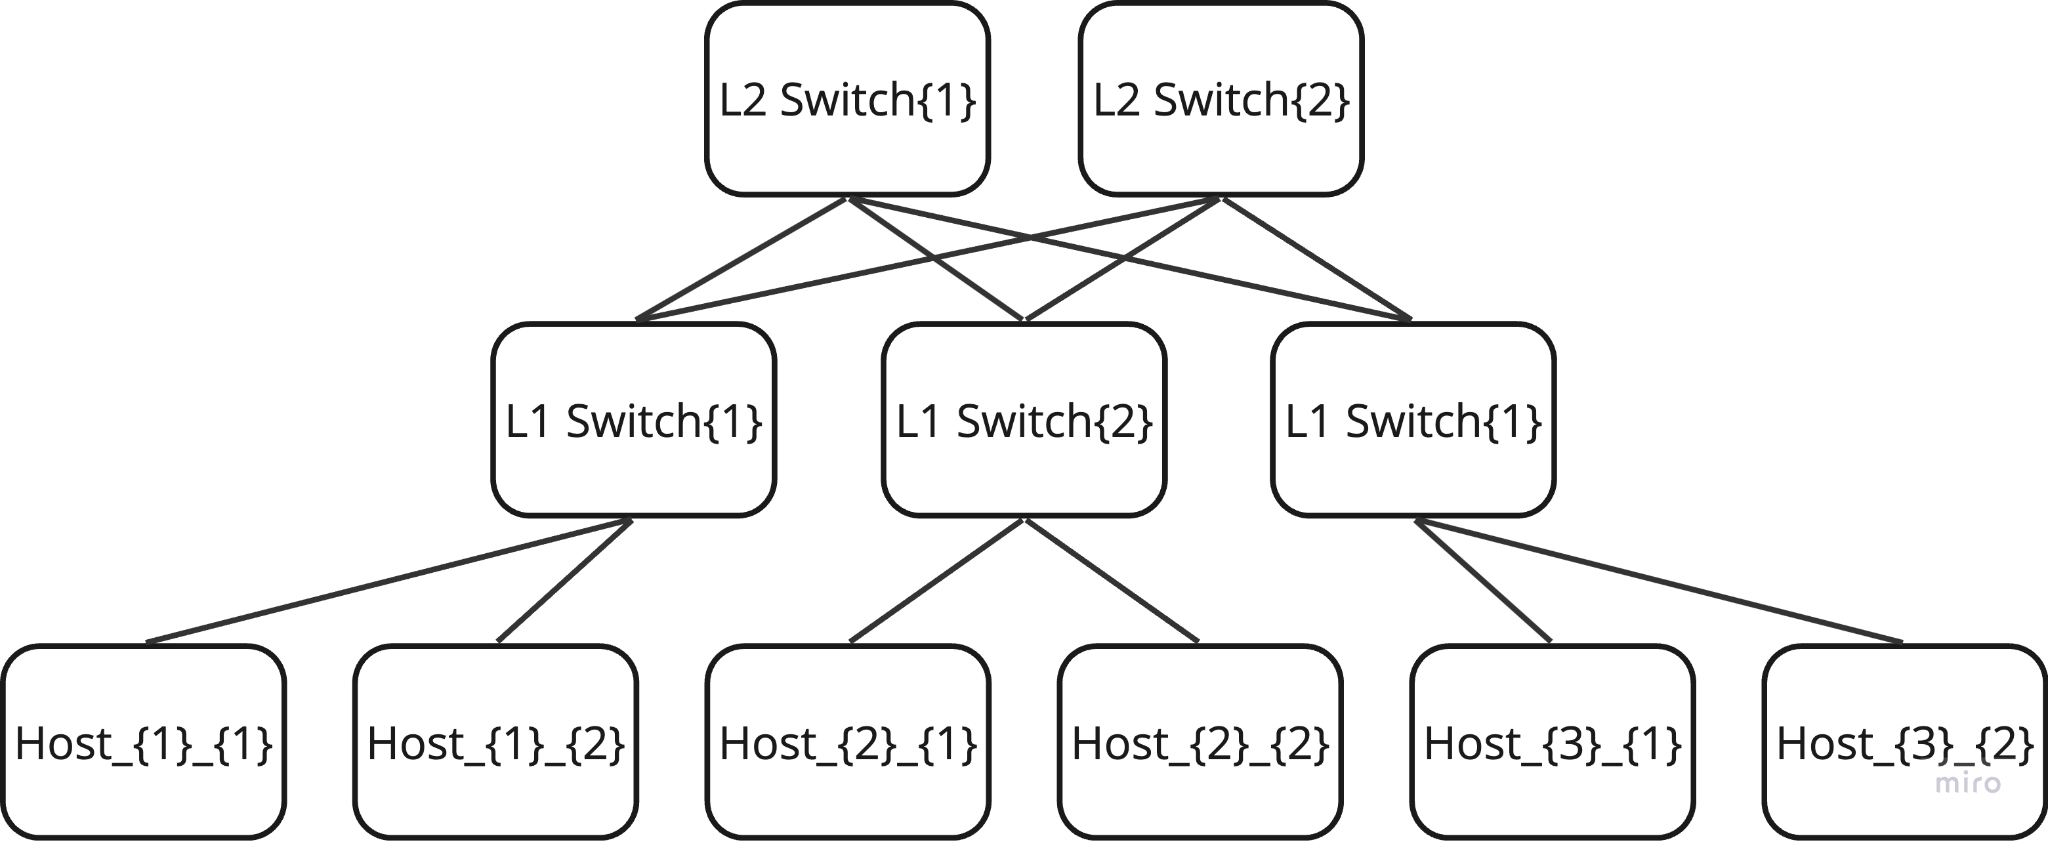
\includegraphics[width=0.8\linewidth]{images/fat_tree_topology}
        \caption{Пример топологии сети <<Fat-Tree>> на 6 серверов по 2 сервера в стойке}
        \label{fig:fat_tree_topology}
    \end{figure}
\end{enumerate}

Подробнее описание модуля \texttt{Network} и примеры использования можно посмотреть в официальной документации \texttt{DSLab}\cite{dslab-network-docs}.

\subsubsection{Модуль хранилища}

Модуль диска используется для симуляции операций чтения-записи в хранилище. Модель предоставляет возможность гибко настроить деградацию производительности диска в зависимости от количества параллельных операций (особенно актуально для HDD операций). Также модель предоставляет возможность реализовать пользовательский планировщик дисковых операций, но по умолчанию используется классический \texttt{<<FIFO>>}-планировщик (First-In-First-Out).  

Подробнее описание модуля \texttt{Storage} и примеры использования можно посмотреть в официальной документации \texttt{DSLab}\cite{dslab-storage-docs}.




\subsection{Вычислительная модель}\label{compute-model}

\subsubsection{Деление на Collection и Execution}\label{sec:execution-collection-model}

Поскольку симулятор может поддерживать несколько разных вычислительных моделей, для описания нагрузки был выбран обобщенный вариант: пользователь описывает задачи (\texttt{Execution}), которые непосредственно запускаются на кластере и потребляют ресурсы, и эти задачи могут быть связаны между собой заданием (\texttt{Collection}). Термин \texttt{Collection} происходит из аналогичного определения задания в последней версии Google Trace\cite{google-clusterdata}. \texttt{Execution} же является минимальной единицей планирования и может из себя представлять как простые вычисления, так и сложную программу, которой для запуска нужно одновременно выделить несколько серверов. Структуры данных представлены в таблицах \ref{tab:execution} и \ref{tab:collection}.

\begin{table}[h]
    \centering
    \label{tab:execution_request_fields}
    \begin{tabular}{|l|l|p{8cm}|}
        \hline
        \textbf{Поле} & \textbf{Тип} & \textbf{Описание} \\
        \hline
        id & \texttt{u64} & Уникальный идентификатор задачи на всю симуляцию \\
        \hline
        collection\_id & \texttt{Option<u64>} & Индекс задания  \\
        \hline
        execution\_index & \texttt{Option<u64>} & Индекс задачи внутри задания \\
        \hline
        time & \texttt{f64} & Время, когда задача становится доступной для планирования \\
        \hline
        schedule\_after & \texttt{Option<f64>} & Время, когда задача становится доступной для исполнения на кластере. Поле введено для поддержки совместимости с трейсом нагрузки из Google. \\
        \hline
        resources & \texttt{ResourceRequirements} & Структура требуемых ресурсов для исполнения задачи \\
        \hline
        profile & \texttt{Rc<dyn ExecutionProfile>} & Профиль нагрузки (см секцию \ref{sec:execution-profile}) \\
        \hline
        wall\_time\_limit & \texttt{Option<f64>} & Максимальное время на выполнение задачи, после которой она автоматически будет отменена \\
        \hline
        priority & \texttt{Option<u64>} & Приоритет задачи \\
        \hline
        start\_after & \texttt{Option<Vec<u64>>} & Список индексов задач внутри задания, после которых можно начать выполнение этой задачи (должен быть указан \texttt{collection\_id}) \\
        \hline
    \end{tabular}
    \caption{Описание структуры данных \texttt{ExecutionRequest}}
    \label{tab:execution}
\end{table}

\begin{table}[h!]
    \centering
    \begin{tabular}{|l|l|p{8cm}|}
        \hline
        \textbf{Поле} & \textbf{Тип} & \textbf{Описание} \\ 
        \hline
        id & \texttt{u64} & Уникальный идентификатор задания на всю симуляцию. \\
        \hline
        time & \texttt{f64} & Время, когда задание приходит на планировщик. \\
        \hline
        user & \texttt{Option<String>} & Пользователь, который запускает задание. Используется для тестирования алгоритмов справедливого разделения кластера. \\
        \hline
        priority & \texttt{Option<u64>} & Приоритет приоритет задания. Если у задачи указан собственный приоритет, то предполагается, что он переопределяет данный приоритет. \\
        \hline
        start\_after\_collection\_ids & \texttt{Option<Vec<u64>>} & Список идентификаторов заданий, после которых можно начать выполнение задач этого задания. \\
        \hline
    \end{tabular}
    \caption{Описание структуры данных \texttt{CollectionRequest}}
    \label{tab:collection}
\end{table}

Описание требуемых ресурсов задачи состоит из требования к количеству хостов, а также опционально к количеству ядер процессора и памяти на хостах. Таким образом, сохраняется возможность поддержать модель планирования аналогичной \texttt{BatSim}, \texttt{IRMaSim} и \texttt{ElastiSim}, но и не упускается возможность для моделирования упаковки задач на кластерах (при указывании количества хостов больше одного,  есть возможность указать требования к ресурсам каждого хоста отдельно или всем сразу).

\subsubsection{ExecutionProfile}\label{sec:execution-profile}

Задачи, которые непосредственно выполняются на кластере, представляются в виде объектов, для которых реализован интерфейс \texttt{ExecutionProfile} (см. рисунок \ref{fig:execution-profile-interface}).

\begin{figure}[h!]
    \small
\begin{rustcode}
#[async_trait(?Send)]
pub trait ExecutionProfile {
  async fn run(self: Rc<Self>, processes: &Vec<HostProcessInstance>);
}
\end{rustcode}
\caption{Интерфейс \texttt{ExecutionProfile}}
\label{fig:execution-profile-interface}
\end{figure}

Метод \texttt{run} может быть реализован самим пользователем, но также могут использоваться заготовки для простых сценариев работы. Такая задача получает в свое <<владение>> от планировщика набор выделенных процессов на узлах кластера и выполняет некоторую работу. Сама работа описывается в терминах асинхронного программирования на Rust и использует предоставленный интерфейс взаимодействия с кластером (рис. \ref{fig:process-cluster-interface}). 
\begin{figure}[h!]
    \footnotesize
\begin{rustcode}
async fn sleep(&self, time: f64);
async fn run_compute_work(&self, compute_work: f64);
async fn transfer_data_process(&self, size: f64, dst_process: ProcessId);
async fn transfer_data_component(&self, size: f64, dst_component: Id);
async fn write_data(&self, size: u64);
async fn read_data(&self, size: u64);
async fn deallocate(&self);
\end{rustcode}
\caption{Интерфейс взаимодействия процессов с кластером}
\label{fig:process-cluster-interface}
\end{figure}

Поскольку симулятор поддерживает несколько моделей вычислений, то интерфейс \\ \texttt{ExecutionProfile} принимает на вход несколько процессов (гарантированно хотя бы один). Количество процессов соответствует количеству серверов, на которых одновременно запущена задача (в соответствии с комплектной моделью планирования). Каждому процессу выделяется аллокация ресурсов на сервере в соответствии с требованиями, и каждый процесс получает асинхронный интерфейс \ref{fig:process-cluster-interface} общения с кластером. Если по ходу выполнения задачи какой-то процесс заканчивает работу раньше других, его можно принудительно завершить через функцию \texttt{deallocate}, освободив ресурсы на сервере. После этого процессом пользоваться будет нельзя (вызов любой другой функции приведет к панике программы).

Для простых ситуаций (например, симуляции нагрузки по Google Trace) используются тривиальные имплементации \texttt{ExecutionProfile}, которые рассчитаны на выполнение на одном сервере (получают на вход ровно один процесс который занимает данные ресурсы на 100\% и спит определенное время).  

Для более сложного моделирования работы задачи можно использовать весь спектр асинхронных инструментов из библиотеки \texttt{futures}\cite{rust-futures}. Например, паттерн работы <<Master-Workers>> можно реализовать как показано на примере \ref{fig:execution-profile-impl}.

Поскольку текущая версия компилятора \texttt{Rust} не поддерживает динамическую диспетчеризацию асинхронных методов, то при реализации интерфейса \texttt{ExecutionProfile} необходимо использовать стороннюю библиотеку \texttt{async-trait}\cite{rust-async-trait}. Удобству использования это не мешает, т.к. все использование библиотеки сводится к добавлению соответствующего макроса к реализации интерфейса.

\begin{figure}[h!]
    \footnotesize 
    \begin{rustcode}
pub struct MasterWorkersProfile {
  pub master_compute_work: f64,
  pub worker_compute_work: f64,
  pub data_transfer_size: f64,
}

#[async_trait(?Send)]
impl ExecutionProfile for MasterWorkersProfile {
  async fn run(self: Rc<Self>, processes: &Vec<HostProcessInstance>) {
    let master = &processes[0];
    let workers = &processes[1..];
    
    futures::future::join_all(workers.iter().map(|p| async {
      master.transfer_data_process(self.data_transfer_size, p.id).await;
      p.run_compute(self.worker_compute_work).await;
    }))
    .await;
    
    master.run_compute(self.master_compute_work).await;
  }
}
    \end{rustcode}
    \caption{Пример реализации интерфейса \texttt{ExecutionProfile}}
    \label{fig:execution-profile-impl}
\end{figure}

\subsubsection{Описание нагрузки через входной файл}

Пользователь может самостоятельно реализовывать свои паттерны нагрузки на кластер, тем самым получая высокую степень точности симуляции. Для использования этих профилей необходимо их зарегистрировать в симуляции перед ее запуском. Тогда можно будет подавать на вход задачи, использующие пользовательские профили. Например, после регистрации профиля \texttt{MasterWorkersProfile} (код \ref{fig:execution-profile-impl}) можно описать задачу (\texttt{ExecutionRequest}) следующим образом c помощью YAML-файла: 

\begin{figure}[h!]
    \footnotesize
    \begin{yamlcode}
                    - submit_time: 10.0
                      resources:
                        nodes_count: 4
                        cpu_per_node: 2
                        memory_per_node: 4
                      profile:
                        type: master-workers
                        args:
                          master_compute_work: 100. 
                          worker_compute_work: 2000. 
                          data_transfer_size: 100.
\end{yamlcode}
    \caption{Пример описания задачи с использованием профиля \texttt{MasterWorkersProfile}}
\end{figure}

Во время симуляции будет создан объект задачи с переданными параметрами (из секции \texttt{args}) и передан в планировщик для размещения на кластере. Как только планировщик найдет для задачи место, будет выполнен метод \texttt{run} из реализации \texttt{MasterWorkersProfile} (см. рисунок \ref{fig:execution-profile-impl}). Поскольку задача будет запущена на 4 серверах одновременно, то в метод \texttt{run} будут переданы 4 процесса. Дальше, следуя коду реализации \ref{fig:execution-profile-impl}, первый процесс станет мастером, а остальные 3 -- рабочими. 

\subsubsection{Декларативное создание профилей нагрузки через файл}

Помимо реализации интерфейса \texttt{ExecutionProfile}, есть и другой способ описания профилей нагрузки -- через YAML-файл. Такой способ описания позволяет проще создавать новые профили нагрузки без необходимости писать код, но с меньшими функциональными возможностями. Пользователю предоставляется два основных комбинатора профилей: параллельный и последовательный, которые могут быть вложены друг в друга. Пример описания профиля нагрузки представлен на рисунке \ref{fig:profile-yaml}. В этом профиле сначала создаются базовые профили нагрузки на вычисления, сеть и диск (рис. \ref{fig:profile-yaml-base}). По сути это введение коротких имен для типовых сценариев нагрузки. В комбинаторах можно использовать как профили с коротким именем, так и профили с аргументами (в том числе пользовательские). Затем создается сложный профиль (рис. \ref{fig:profile-yaml-complex}) с таким сценарием работы: 
\begin{enumerate}
  \item На всех процессах происходит чтение данных с диска, затем все процессы делают простые вычисления (\texttt{compute-simple}).
  \item Все процессы параллельно делают сложное вычисление и общаются по сети в соответствии с профилем \texttt{net-all-to-all-simple}.\item Все процессы записывают результаты на диск. 
  \item Снова параллельные простые вычисления на всех процессах и общение по сети.
  \item В конце запись данных на диск всеми процессами.
\end{enumerate}

Вся последовательность повторяется дважды. 

\begin{figure}[h!]
    \footnotesize
\begin{subfigure}{0.5\textwidth}
    \begin{yamlcode}
    compute-simple: 
      type: compute-homogenous
      args: 
        compute_work: 1000.0 
    compute-hard:
      type: compute-homogenous
      args:
        compute_work: 2000.0
    net-all-to-all-simple:
      type: communication-homogenous
      args: 
        size: 500.0 
    disk-simple-read: 
      type: disk-read 
      args: 
        size: 1000
    disk-simple-write-part: 
      type: disk-write 
      args: 
        size: 600  
    \end{yamlcode}
    \caption{Пример описания базовых профилей}
    \label{fig:profile-yaml-base}
\end{subfigure}
\begin{subfigure}{0.5\textwidth}
    \begin{yamlcode}
complex_execution_profile:
  type: sequence
  args:
    repeat: 2
    profiles:
      - disk-simple-read
      - compute-simple
      - parallel
        args:
          profiles:
            - compute-hard
            - net-all-to-all-simple
      - disk-simple-write-part
      - parallel
        args:
          profiles:
            - compute-simple
            - net-all-to-all-simple
      - disk-simple-write-part
\end{yamlcode}
    \caption{Пример описания профиля через комбинаторы}
    \label{fig:profile-yaml-complex}
\end{subfigure}
\caption{Пример описания профилей нагрузки через YAML-файл}
\label{fig:profile-yaml}
\end{figure}

Можно видеть, что вложенные комбинаторы позволяют создавать сложные сценарии. По умолчанию предоставляются базовые профили, описанные в таблице \ref{tab:default-profiles}. Эти профили покрывают функциональность профилей из \texttt{BatSim}\cite{batsim-profile-types-overview} и позволяют создавать разнообразные сценарии нагрузки на кластер, а с помощью комбинаторов можно сделать более сложные вложенные профили. Более того, к такому декларативному описанию задач можно добавить и собственные профили, которые реализуют интерфейс \texttt{ExecutionProfile} (см. секцию \ref{sec:execution-profile}). Определенные профили могут использовать в качестве зависимостей только те профили, которые была определены выше по файлу, это исключает возможность возникновения циклических зависимостей. 

\begin{table}[h!]
    \centering
    \begin{tabular}{|l|l|p{7cm}|}
        \hline
        \textbf{Профиль} & \textbf{Аргументы} & \textbf{Описание} \\ 
        \hline
        compute-homogenous & \texttt{compute\_work: f64} & Выполнить \texttt{compute\_work} работы на всех переданных процессах.\\
        \hline
        compute-matrix &  \texttt{matrix: Vec<Vec<f64>>} & Выполнить вычисления на процессах согласно матрице \texttt{matrix}, например: 
        [10, 20] -- первый процесс выполняет работу 10, а второй -- 20. \\
        \hline
        \makecell{
        communication-\\homogenous} & \texttt{size: f64} & Передать \texttt{size} данных между всеми переданными процессами. \\
        \hline 
        communication-matrix &  \texttt{matrix: Vec<Vec<f64>>}  & Передать данные между процессами согласно матрице \texttt{matrix}, например: 
        [0, 20,
        10, 0] -- первый процесс передает второму данные размера 20, а второй первому -- 10. Аналогично с определением матрицы передачи данных из \texttt{BatSim}\cite{batsim-profile-types-overview}. \\
        \hline
        communication-src-dst & \makecell[tl]{
              \texttt{src: Vec<usize>} \\ \texttt{dst: Vec<usize>} \\ \texttt{size: f64} }
         & Передать \texttt{size} данных от процессов с индексами из \texttt{src} к процессам с индексами из \texttt{dst}. \\
        \hline
        \makecell{communication-\\external} & \makecell[tl]{
             \texttt{processes: Vec<usize>}\\ \texttt{input\_size: f64}\\ \texttt{output\_size: f64}\\ \texttt{component\_name: String}} & Передать данные между процессами и другими компонентами сети, например, между процессами и внешним хранилищем. Для этого внешнее хранилище должно быть предварительно зарегистрировано в сети и настроено. \\
            \hline
        disk-read & \makecell[tl]{ \texttt{processes: Vec<usize>}\\ \texttt{size: f64}} & Прочитать \texttt{size} данных с диска у данных процессов. Если процессы не указаны, чтение происходит у всех. \\
        \hline
        disk-write & \makecell[tl]{\texttt{processes: Vec<usize>}\\\texttt{size: f64}}  & Записать \texttt{size} данных на диск у данных процессов. Если процессы не указаны, запись на диск происходит у всех. \\
        \hline
    \end{tabular}
    \caption{Описание предоставляемых по умолчанию профилей нагрузки}
    \label{tab:default-profiles}
\end{table}

\subsection{Модель планирования заданий}

Симулятор поддерживает несколько основных моделей планирования: 
\begin{enumerate}
    \item Планировщик принимает решение о планировании на основе всей информации (выбирает подходящую задачу и подходящий хост). В таком случае планировщик может вызываться периодически и по событиям (например, по получению новых задач и завершению прошлых). В такой модели у планировщика есть набор задач, которые в данный момент наиболее приоритетны (обычно это некоторая очередь), и планировщик выбирает под эти задачи наиболее подходящие серверы (или части серверов) кластера. Такая модель используется в одном из наиболее популярных планировщиков для кластеров \texttt{Slurm}(Simple Linux Utility for Resource Management)\cite{slurm-cpu-management}. В этой модели под задание (job) с помощью отдельного плагина \texttt{Node Selection} выбирается набор серверов, на которые впоследствии распределяются задачи (tasks). 
    \item Вычислительные серверы периодически сообщают планировщику о своих свободных ресурсах, и планировщик принимает решение о подходящих задачах (которые могут аналогичным образом браться из очереди) конкретно под сервер, который сделал запрос. Также серверы информируют планировщик об изменении свободных ресурсов в связи с завершением текущих задач. Такая модель используется в планировщике кластера YT в Яндексе\cite{yt-scheduler}.
\end{enumerate}

Благодаря поддержке обеих моделей симулятор способен воспроизводить работу разных планировщиков, что делает его более универсальным. Однако, из-за этого размывается четкое разделение рабочей нагрузки на задание (job) и задачи (tasks). В такой ситуации получается, что \texttt{Execution} (см. раздел \ref{sec:execution-collection-model}) может выступать как простейшая задача продолжительностью несколько минут (из модели планировщика \texttt{YT}, \texttt{Google} и др.), так и сложная много-серверная программа, внутри которой есть своя собственная логика разделения ресурсов (из модели планировщика \texttt{Slurm} и симулятора \texttt{BatSim}). В последнем случае дополнительную логику <<планирования>> и разделения большого объема выделенных ресурсов реализует как раз сам пользователь внутри \texttt{ExecutionProfile}.


Реализуя свой планировщик пользователь может реализовать интерфейс планировщика \texttt{Scheduler} (см. рисунок \ref{fig:scheduler-interface}). 

\begin{figure}[h!]
    \footnotesize
    \begin{rustcode}
pub trait Scheduler {
  fn on_host_added(&mut self, ctx: &Context, host: HostConfig);
  fn on_execution_request(&mut self, ctx: &Context, req: ExecutionRequest);
  fn on_collection_request(&mut self, ctx: &Context, req: CollectionRequest);
  fn on_execution_finished(&mut self, ctx: &Context, execution_id: u64);
  fn on_host_notification(&mut self, ctx: &Context, host_id: Id, resources: ResourcesPack);
}
    \end{rustcode}
    \caption{Интерфейс планировщика \texttt{Scheduler}}
    \label{fig:scheduler-interface}
\end{figure}

С помощью контекста (который передается в каждый метод интерфейса \ref{fig:scheduler-interface}) планировщик получает доступ к генератору псевдослучайных чисел и управляет симуляцией: ставит на исполнение задачи, выбрав для них набор серверов и частично отменяет их. Полная отмена в данный момент не полностью реализована, например невозможно отменить операцию передачи данных по сети, это связано с внутренними ограничениями  модуля \texttt{dslab\_network}, которые в будущем могут быть доработаны.

Для более точного управления моделью планировщика можно запустить симуляцию, передав ей отдельный компонент симуляции \texttt{DSLab}, который будет получать сырые события от компонентов \texttt{Proxy} (о новых задачах) и \texttt{Cluster} (о свободных ресурсах и завершенных задачах). Тогда у пользователя будет еще больше контроля над моделью планирования: компонент-планировщик сможет отправлять себе произвольные события, использовать асинхронные функции из асинхронного расширения ядра \texttt{DSLab} и т.д. Это качественно выделяет разработанный симулятор от аналогов, т.к. другие симуляторы предлагают только \texttt{callback} модель, где пользователь пишет обработку всех типов событий, приходящих от кластера. В новом симуляторе же есть возможность использовать асинхронное расширение ядра \texttt{DSLab} и реализовать программу-планировщик на качественно другом уровне. Подробнее о преимуществах этого функционала можно прочитать в работе о добавлении асинхронности в \texttt{DSLab}\cite{async-dslab}.



\subsection{Входные данные симуляции}

\subsubsection{Трейс нагрузки}\label{sec:input-format-trace}

В качестве входных данных симуляции выступает трейс нагрузки на кластер. Трейс представляет собой набор задач, которые поступают на кластер в течение симуляции. Как описывалось в разделе \ref{sec:execution-collection-model}, они могут быть связаны некоторым общим заданием. В данный момент симулятор поддерживает несколько видов входной нагрузки: 

\begin{itemize}
   \item \texttt{Native} -- трейса нагрузки в формате \texttt{YAML}, описанного в секции \ref{compute-model}. Состоит из нескольких файлов: файл с описанием задач (\texttt{ExecutionRequest}-ы), файл с описанием заданий (\texttt{CollectionRequest}-ы) и файл с описанием профилей нагрузки (\texttt{ExecutionProfile}).
   \item \texttt{Google} -- трейс нагрузки кластера \texttt{Google}\cite{google-clusterdata}. Версия 2019 года представлена в виде таблицы \texttt{BigQuery}, из которой достаточно сложно скачать большой объем данных (из-за ограниченных квот), однако версию 2011 года можно скачать в виде \texttt{CSV}-файла. Подробное описание и сравнение этих трейсов представлено в статье \texttt{Borg: Next Generation}\cite{borg-next-gen} от Google. Для простоты в симуляторе предполагается, что все задачи потребляют все выделенные ресурсы на протяжении всего времени выполнения (заполняются тривиальными заглушками \texttt{ExecutionProfile}), однако в трейсе 2019 года присутствует подробная информация о профиле загрузки задачи, которую можно использовать для более точного моделирования в последующей работе. Сам трейс представлен в виде событий, поэтому его инкрементальное прочтение сделать сложно (для того, чтобы выяснить время выполнение задачи, необходимо прочитать трейс до события окончания задачи), из-за этого с трейсом удобнее работать, преобразовав его в формат \texttt{Native}. Поскольку данные о требованиях к ресурсам задач представлены в нормированном виде (числами с плавающей точкой от 0 до 1, где 1 -- максимальное возможное значение ресурса среди всех доступных серверов), то при чтении этого трейса необходимо указать константу, на которую умножаются эти значения, чтобы получить целочисленные значения CPU и памяти. 
   \item \texttt{Alibaba} -- Трейс нагрузки кластера \texttt{Alibaba} 2018 года\cite{alibaba-clusterdata}. Состоит из двух файлов: файл \texttt{batch\_tasks.csv} описывает зависимости между выполняемыми задачами (\texttt{instances}), информация о которых содержится в \texttt{batch\_instances.csv}. Информация о задачах по аналогии с Google Trace переводится в тривиальные профили нагрузки. Однако, этот трейс можно читать инкрементально, что упрощает работу с ним.  
   \item \texttt{Standard Workload Format Reader} -- Трейс нагрузки в формате \texttt{SWF}\cite{standard-workload-format}. Транслируется в симулятор по аналогии с Alibaba Trace, т.к. может быть в исходном виде прочитан инкрементально. 
   \item \texttt{Random Trace Generator}. Детерминированный генератор синтетической нагрузки на кластер. С помощью встроенного в симуляцию \texttt{DSLab} генератора случайных чисел создает заданное количество задач с заданными требованиями к ресурсам. Время выполнение (либо необходимая процессорная работа) генерируется из нормального распределения с заданными параметрами среднего и дисперсии (см. пример в секции \ref{sec:example-fairness}).

\end{itemize}

Все перечисленные генераторы нагрузки реализуют интерфейс \texttt{WorkloadGenerator} (см. \ref{fig:workload-generator-trait}). Поскольку количество задач может быть очень большим (входные файлы могут иметь размеры десятки гигабайт) и не поместится в оперативную память сразу, то генераторы нагрузки должны уметь читать данные инкрементально, выдавая задачи для планировщика пачками не больше указанного лимита. Предполагается, что задачи в трейсе упорядочены по времени поступления на кластер. 
\begin{figure}[h!]
    \footnotesize
\begin{rustcode}
pub trait WorkloadGenerator {
  fn get_workload(
    &mut self, ctx: &SimulationContext, limit: Option<u64>,
  ) -> Vec<ExecutionRequest>;
  
  fn get_collections(&self, ctx: &SimulationContext) -> Vec<CollectionRequest>;
}
\end{rustcode}
    \caption{Интерфейс \texttt{WorkloadGenerator}}
    \label{fig:workload-generator-trait}
\end{figure}

Пользователь может реализовать этот интерфейс самостоятельно и тогда у него появится возможность использовать свой собственный формат трейса нагрузки. Как альтернативный вариант, можно конвертировать имеющийся трейс в один из поддерживаемых форматов.

\subsubsection{Конфигурация кластера и сети}

Существует несколько способов задать конфигурацию серверов в кластере: 
\begin{enumerate}
    \item Через конфигурационный файл в формате YAML. Пример конфигурации представлен на рисунке \ref{fig:example-sim-config}. Есть возможность задать группы серверов с одинаковой конфигурацией, а затем получать статистику утилизации ресурсов в серверах по группам (подробнее см. раздел \ref{sec:output-monitoring}). Составные части каждого сервера описаны в разделе \ref{cluster-model}. Через конфигурацию также можно указать вид сети, используемой в кластере, и ее параметры (например, указать распределение хостов по стойкам при использовании топологии \texttt{Fat-Tree}) (описана в разделе \ref{sec:network-model}).
    \item Через чтение конфигурации кластера из \texttt{Google-trace}.
    \item Через чтение конфигурации кластера из \texttt{Alibaba-trace}.
\end{enumerate}

Стоит отметить, что использование трейса нагрузки из какого-либо источника (\texttt{Google trace} или \texttt{Alibaba trace}) не обязывает использовать конфигурацию кластера из этого же источника и наоборот. Однако, учитывая, что в обоих трейсах информация о ресурсах является нормированной (в целях скрыть данные о реальных мощностях кластера и объеме выполняемых задач), использовать их как-то иначе представляется практически невозможным. 

\subsection{Выходные данные симуляции}\label{sec:output-monitoring}

Выходными данными симуляции являются файлы с метриками загруженности кластера и очереди задач. В процессе работы отдельный компонент \texttt{Monitoring} собирает данные о мгновенной загрузке серверов и размере очереди, и агрегирует их, считая среднее значение на заданных временных промежутках. Пользователь может настроить интервал сжатия данных в конфигурационном файле симуляции (см. конфигурацию \ref{fig:example-sim-config}). В разделе справедливости распределение ресурсов по умолчанию собираются метрики использования доминантной доли ресурса различными пользователями\cite{drf-article}. Подробнее это рассмотрено в примере использования симулятора \ref{sec:example-fairness}. По полученным файлам в формате \texttt{CSV} можно проводить анализ данных и строить графики, например с помощью известных библиотек \texttt{Python}: \texttt{pandas} и \texttt{matplotlib}. 

\subsection{Конфигурация симуляции}

Вся настройка параметров симуляции происходит через конфигурационный файл в формате YAML. Пример конфигурации представлен на рисунке \ref{fig:example-sim-config}. 

\begin{figure}[h!]
    \footnotesize
    \begin{yamlcode}
                    workload:
                      - type: Native
                        path: /path/to/trace
                        options: 
                          profiles_path: /path/to/profiles
                    
                    hosts: 
                      - count: 5
                        cpus: 20
                        memory: 20
                        name_prefix: c
                      - count: 5
                        cpus: 5
                        memory: 60
                        name_prefix: m
                    
                    monitoring:
                      host_load_compression_time_interval: 100
                      scheduler_queue_compression_time_interval: 100
                      display_host_load: false 
                      collect_user_queues: true
                      output_dir: /path/to/output_dir
                    
                    scheduler:
                      hosts_invoke_interval: 10
\end{yamlcode}
\caption{Пример конфигурации симуляции}
\label{fig:example-sim-config}
\end{figure}

В такой симуляции входная нагрузка будет в формате \texttt{Native} с указанными дополнительными профилями нагрузки. Используются два типа серверов: 5 серверов с 20 ядрами CPU и 20 Гб памяти и 5 серверов с 5 ядрами CPU и 60 Гб памяти. Сбор статистики загруженности кластера ведется только по группам и целиком на кластер, а также собираются метрики справедливости планирования (по пользователям). Метрики загруженности и размера очереди сжимаются на отрезках времени в 100 единиц и берется среднее на каждом отрезке. Каждый хост сообщает о свободных ресурсах планировщику каждые 10 единиц времени (единицы измерения могут быть любыми, но по умолчанию подразумеваются секунды). 

\subsection{Параллельный запуск нескольких симуляций}

Для более быстрой параллельной проверки нескольких гипотез можно воспользоваться функциональностью параллельного запуска симуляций. Для каждой симуляции необходимо предоставить отдельный конфигурационный файл. Во избежании конфликтов важно, чтобы выходные данные записывались в разные директории (это тоже можно указать в конфигурации). Пример использования параллельного запуска симуляций можно смотреть в примерах репозитория с симулятором\cite{dslab-cluster-scheduling-parallel-launching}.


\section{Эксперименты и тестирование}\label{sec:experiments}

\subsection{Производительность}\label{sec:experiments-speed}

В рамках эксперимента на производительность симуляции был взят \texttt{Alibaba-trace} 2018 года\cite{alibaba-clusterdata}. Трейс описывает загрузку кластера из 4000 серверов в течении 8 дней и содержит 1.5 миллиарда задач. Суммарный объем файла с задачами составляет 105GB. Для симуляции было взято подмножество задач первых двух с половиной дней (около 380 миллионов задач), входной файл занимает 25GB. Благодаря инкрементальному чтению трейса, нет необходимости загружать все данные в оперативную память сразу. Время работы симулятора в зависимости от количества входных задач представлена на графике \ref{fig:speed-test}. 
% Замеры производились на компьютере MacBook Air с процессором M3. Поскольку у такого компьютера нет активного охлаждения, то при длительной симуляции (больше минуты) производительность падает из-за перегрева.
Видно, что рост времени работы линейный от количества задач.

Получается, что на симуляцию кластера в течение двух с половиной дней (220000 секунд) ушло 2600 секунд (около 45 минут). Таким образом получаем коэффициент ускорения в 85 раз (по сравнению с реальным временем работы кластера). При этом использовался простейший алгоритм планирования, время работы которого не зависит от количества задач в очереди, и который старается максимально загрузить все имеющиеся ресурсы. Стоит отметить, что от эффективности работы пользовательского алгоритма планирования напрямую зависит и время работы симулятора. Если задачи будут слишком быстро накапливаться и не будут планироваться на кластер (и, соответственно, уничтожаться по завершению), то это приведет к резкому росту потребления оперативной памяти программой-симулятором, т.к. инкрементальное чтение задач из трейса происходит согласно внутреннему времени симуляции.

Еще одной проблемой при запуске таких больших симуляций является необходимость подать на вход симулятору файл с задачами отсортированными по времени поступления в планировщик, однако опубликованные трейсы обычно не отсортированы. Поэтому перед запуском необходимо решить задачу сортировки большого \texttt{CSV} файла во внешней памяти. 

\begin{figure}[h!]
  \centering 
  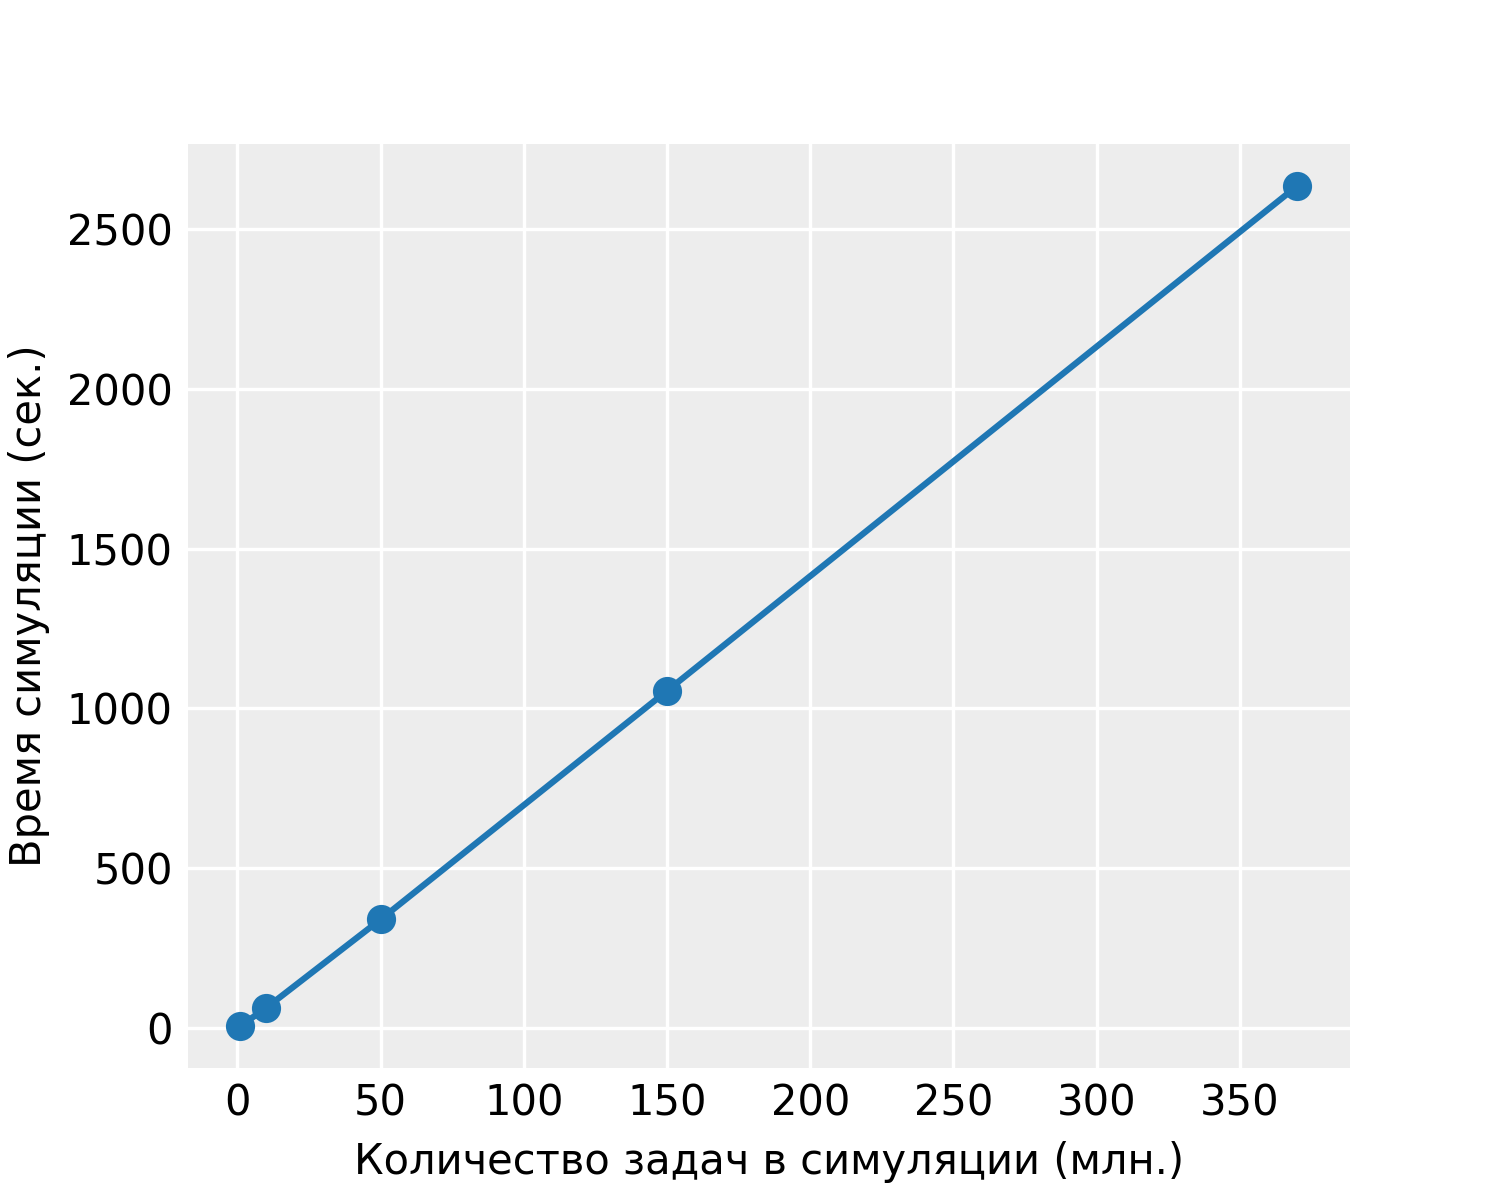
\includegraphics[width=0.8\linewidth]{images/simulation_time}
  \caption{Время работы симуляции в зависимости от количества задач}
  \label{fig:speed-test}
\end{figure}

При сравнении производительности симуляции с другими симуляторами был проведен замер сравнение времени работы на нагрузке из 200000 простых независимых задач. Симулятор \texttt{AccaSim} справился с работой за 25 секунд, а симулятор на основе \texttt{DSLab} -- за 2.5 секунды. Таким образом, симулятор на основе \texttt{DSLab} работает в 10 раз быстрее, чем \texttt{AccaSim}. Это связано с тем, что \texttt{AccaSim} реализован на языке \texttt{Python}, который существенно уступает в производительности языку \texttt{Rust}. Симуляторы \texttt{BatSim}, \texttt{IRMaSim} и \texttt{ElastiSim} не поддерживают инкрементальное чтение трейса нагрузки, поэтому запуск таких больших симуляций в них не представляется возможным (из-за слишком большого одновременного потребления оперативной памяти). Это нельзя назвать однозначным недостатком, ведь эти симуляторы фокусируются на другой, более узкой области -- точное моделирование сложных задач и сети.  

\subsection{Справедливость}\label{sec:example-fairness}

В качестве тестирования симулятора были проведены эксперименты на известный алгоритм справедливого распределения кластера между несколькими пользователями. Были реализованы алгоритмы \texttt{DRF}\cite{drf-article} и \texttt{Tetris}\cite{tetris-article}. 

Алгоритм DRF (Dominant Resource Fairness) основан на понятии доминантного ресурса пользователя. Если пользователь потребляет 1/10 всей памяти в кластере, 1/15 всех ядер процессора, то для него доминантной долей будет считаться число 1/10 (в ситуации, когда распределяется два доступных ресурса -- CPU и RAM). Смысл алгоритма состоит в том, чтобы каждый пользователь получал равную доминантную долю ресурсов (в случае, когда квоты пользователей равны, иначе доля считается от выделенной на кластере квоты). Поэтому из всех задач, которые готовы к исполнению планировщик в каждый момент времени выбирает самого обделенного пользователя и запускает его задачу. 

Такой подход позволяет обеспечить справедливое распределение ресурсов, однако упаковка задач на серверах может быть неоптимальной. Для борьбы с этим был предложен алгоритм \texttt{Tetris}\cite{tetris-article}. На вход принимается произвольная функция справедливости (в нашем случае это DRF), а также <<коэффициент справедливости>> $f \in [0, 1]$. В каждый момент принятия решения, планировщик сортирует задачи по приоритету их размещения на кластере с точки зрения справедливости, а затем выбирает наилучшую задачу с точки зрения упаковки среди $(1 - f)$ доли очереди. В качестве эвристической функции упаковки \texttt{Tetris} использует скалярное произведение вектора ресурсов задачи на вектор свободных ресурсов сервера. Чем оно больше, тем лучше задача упаковывается на сервер. В таком виде приоритет явно отдается более тяжелым задачам, чтобы этого избежать, можно разделить результат на нормы векторов ресурсов. 

Таким образом, конфигурируя алгоритм через параметр $f$, можно добиться баланса между справедливостью и плотностью упаковки задач. При $f = 0$ на каждом шаге планировщик выбирает наиболее подходящую задачу с точки зрения упаковки (т.к. выбирает среди всей доступной очереди), а при $f = 1$ выбирает наиболее обделенного пользователя (т.к. может взять только первую задачу из очереди). Стоит отметить, что при любых значениях $f < 1$ справедливость распределения ресурсов не гарантируется и существует возможность развития событий, при котором один из пользователей оказывается полностью обделен ресурсами на кластере, т.к. его задачи всегда подходят хуже других. На практике (при значении $f$ достаточно близком к 1) такое случается крайне редко из-за очень большого количества задач с различными требованиями. 

Для такой симуляции был выбран кластер с распределением ресурсов по серверам, указанными на графике \ref{fig:cluster-resources-distribution}.

\begin{figure}[h!]
    \centering 
    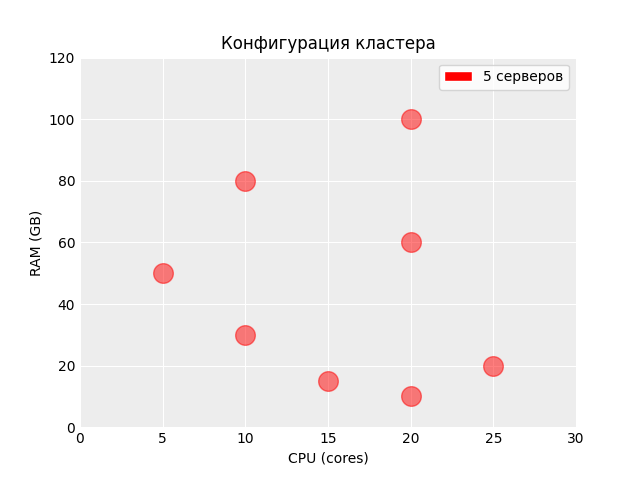
\includegraphics[width=0.7\linewidth]{images/hosts_distribution}
    \caption{Распределение ресурсов на серверах кластера}
    \label{fig:cluster-resources-distribution}
\end{figure}

В качестве синтетической нагрузки были сгенерированы 10 пользователей с равной долей доступа к кластеру с запросами на задачи, представленными в таблице \ref{tab:tasks_load_description}. Каждый пользователь непрерывно поставлял задачи со своими фиксированными требованиями (CPU и RAM). Продолжительность задачи генерировалась из нормального распределения с параметрами среднего (\texttt{duration mean}) и дисперсии (\texttt{duration dev}) для каждого пользователя. 

\begin{table}[h!]
    \centering
    \begin{tabular}{|c|c|c|c|c|c|}
        \hline
        \textbf{Пользователь} & \textbf{CPU} & \textbf{RAM} & \textbf{Количество задач} & \textbf{Duration Mean} & \textbf{Duration Dev} \\
        \hline
        user0 & 1 & 5 & 1500 & 250 & 40 \\
        \hline
        user1 & 1 & 10 & 800 & 400 & 40 \\
        \hline
        user2 & 1 & 15 & 800 & 300 & 30 \\
        \hline
        user3 & 2 & 5 & 1300 & 250 & 30 \\
        \hline
        user4 & 2 & 6 & 1200 & 250 & 30 \\
        \hline
        user5 & 2 & 7 & 800 & 300 & 40 \\
        \hline
        user6 & 5 & 4 & 1000 & 180 & 30 \\
        \hline
        user7 & 5 & 5 & 700 & 160 & 10 \\
        \hline
        user8 & 7 & 5 & 200 & 800 & 200 \\
        \hline
        user9 & 10 & 2 & 400 & 220 & 30 \\
        \hline
    \end{tabular}
    \caption{Описание синтетической нагрузки на кластер}
    \label{tab:tasks_load_description}
\end{table}


При симуляции с разными параметрами справедливости производились замеры средней утилизации кластера от момента полной загрузки кластера до момента, когда у какого-либо пользователя заканчивались задачи. Результаты представлены на графиках \ref{fig:utilization-results}.

\begin{figure}[h!]
    \centering 
    \begin{subfigure}{0.49\linewidth}
        \centering
        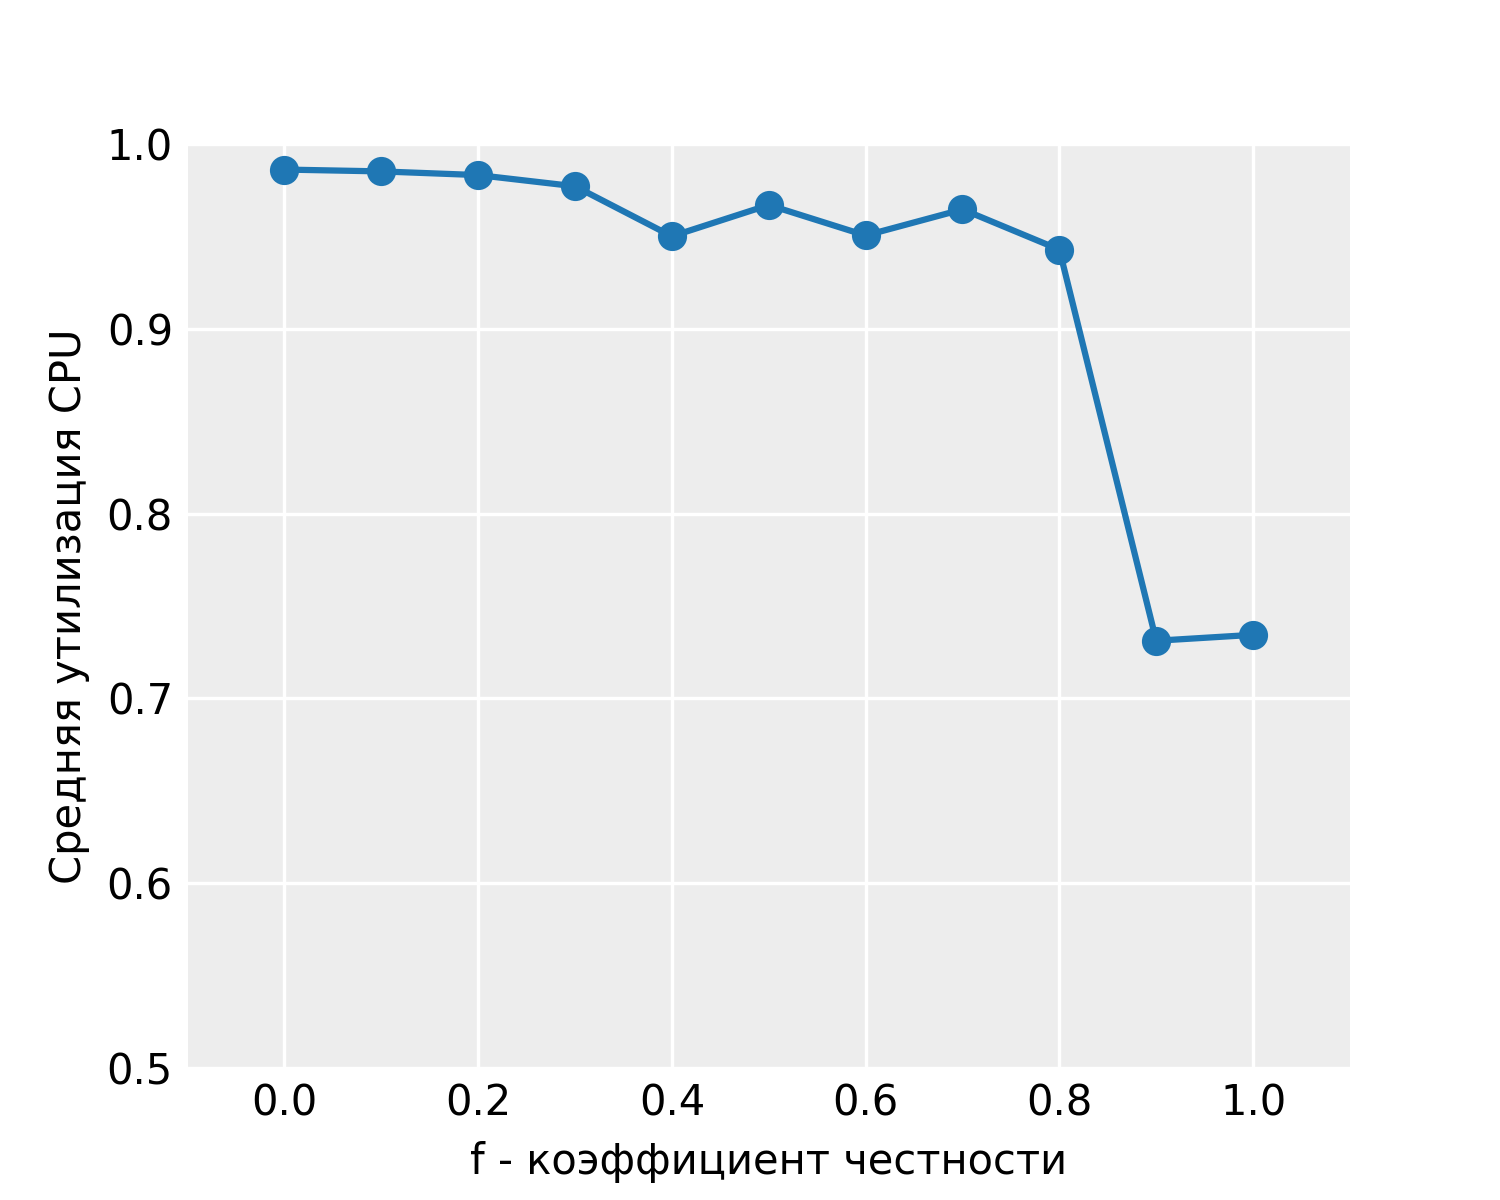
\includegraphics[width=\linewidth]{images/cpu_utilization}
        \caption{Утилизация CPU в зависимости от $f$}
    \end{subfigure}
    \begin{subfigure}{0.49\linewidth}
        \centering
        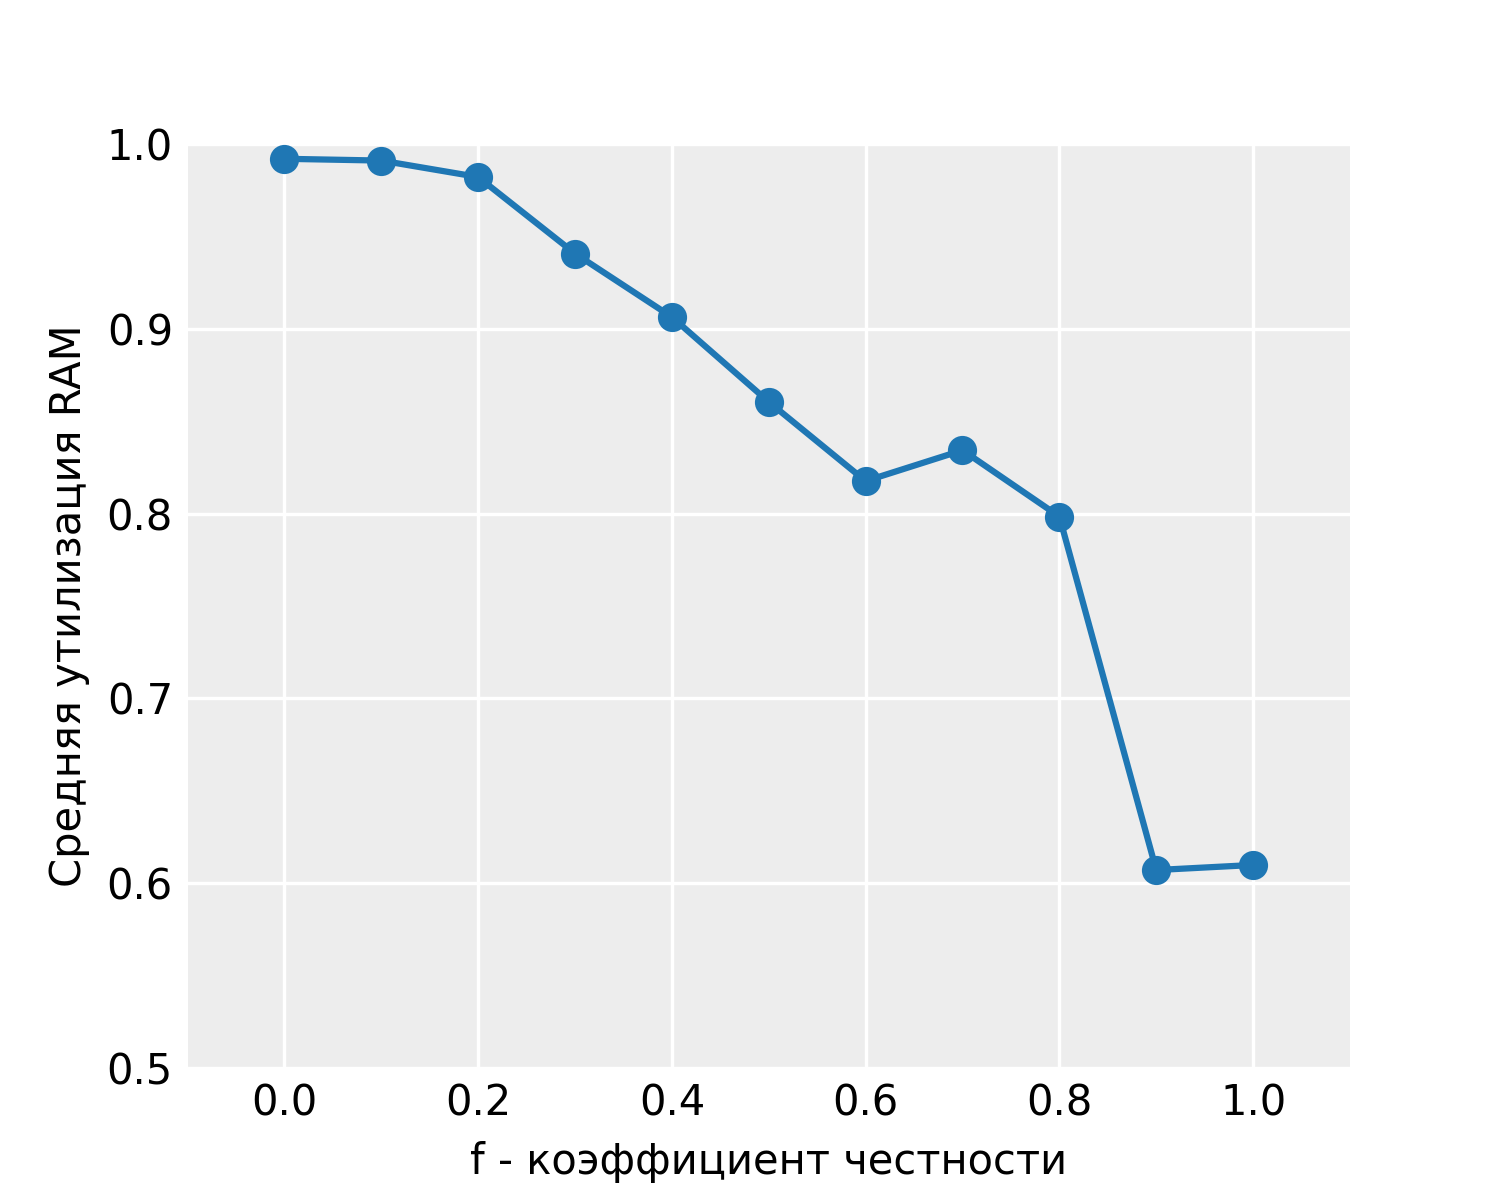
\includegraphics[width=\linewidth]{images/memory_utilization}
        \caption{Утилизация памяти в зависимости от $f$}
    \end{subfigure}
    \caption{Утилизация кластера в зависимости от параметра справедливости}
    \label{fig:utilization-results}
\end{figure}

Из графиков видно, что качественный скачок в утилизации происходит при значении параметра справедливости $f = 0.8$. Это можно объяснить тем, что ровно при этом значении параметра, алгоритм \texttt{Tetris} получает возможность выбирать из двух задач при планировании (т.к. всего пользователей 10). Как только появляется такая возможность, качество упаковки задач на кластере резко возрастает. 

Чтобы сравнить справедливость распределения, посмотрим на графики \ref{fig:fairness-results} доминантных долей пользователей в течение времени симуляции. Можно отметить, что при коэффициенте $f = 0.6$ (график \ref{fig:fair_share_06}) справедливость страдает не сильно, особенно пока у всех пользователей есть задачи, а при $f = 0.5$ (график \ref{fig:fair_share_05}) уже можно видеть, что два пользователя существенно обделяются (получают долю в два раза меньше, чем получает большинство), еще два других пользователя обделяются не так сильно.  На обоих графиках видно, что самым обделенным пользователем является \texttt{user9} -- это можно объяснить тем, что у него профиль нагрузки задач отличается больше всех от других: он потребляет больше всех \texttt{CPU} и меньше всех \texttt{RAM}, поэтому его задачи хуже всего подходят в освободившиеся слоты от других пользователей. 


\begin{figure}[h!]
    \centering 
    \begin{subfigure}{0.49\linewidth}
        \centering
        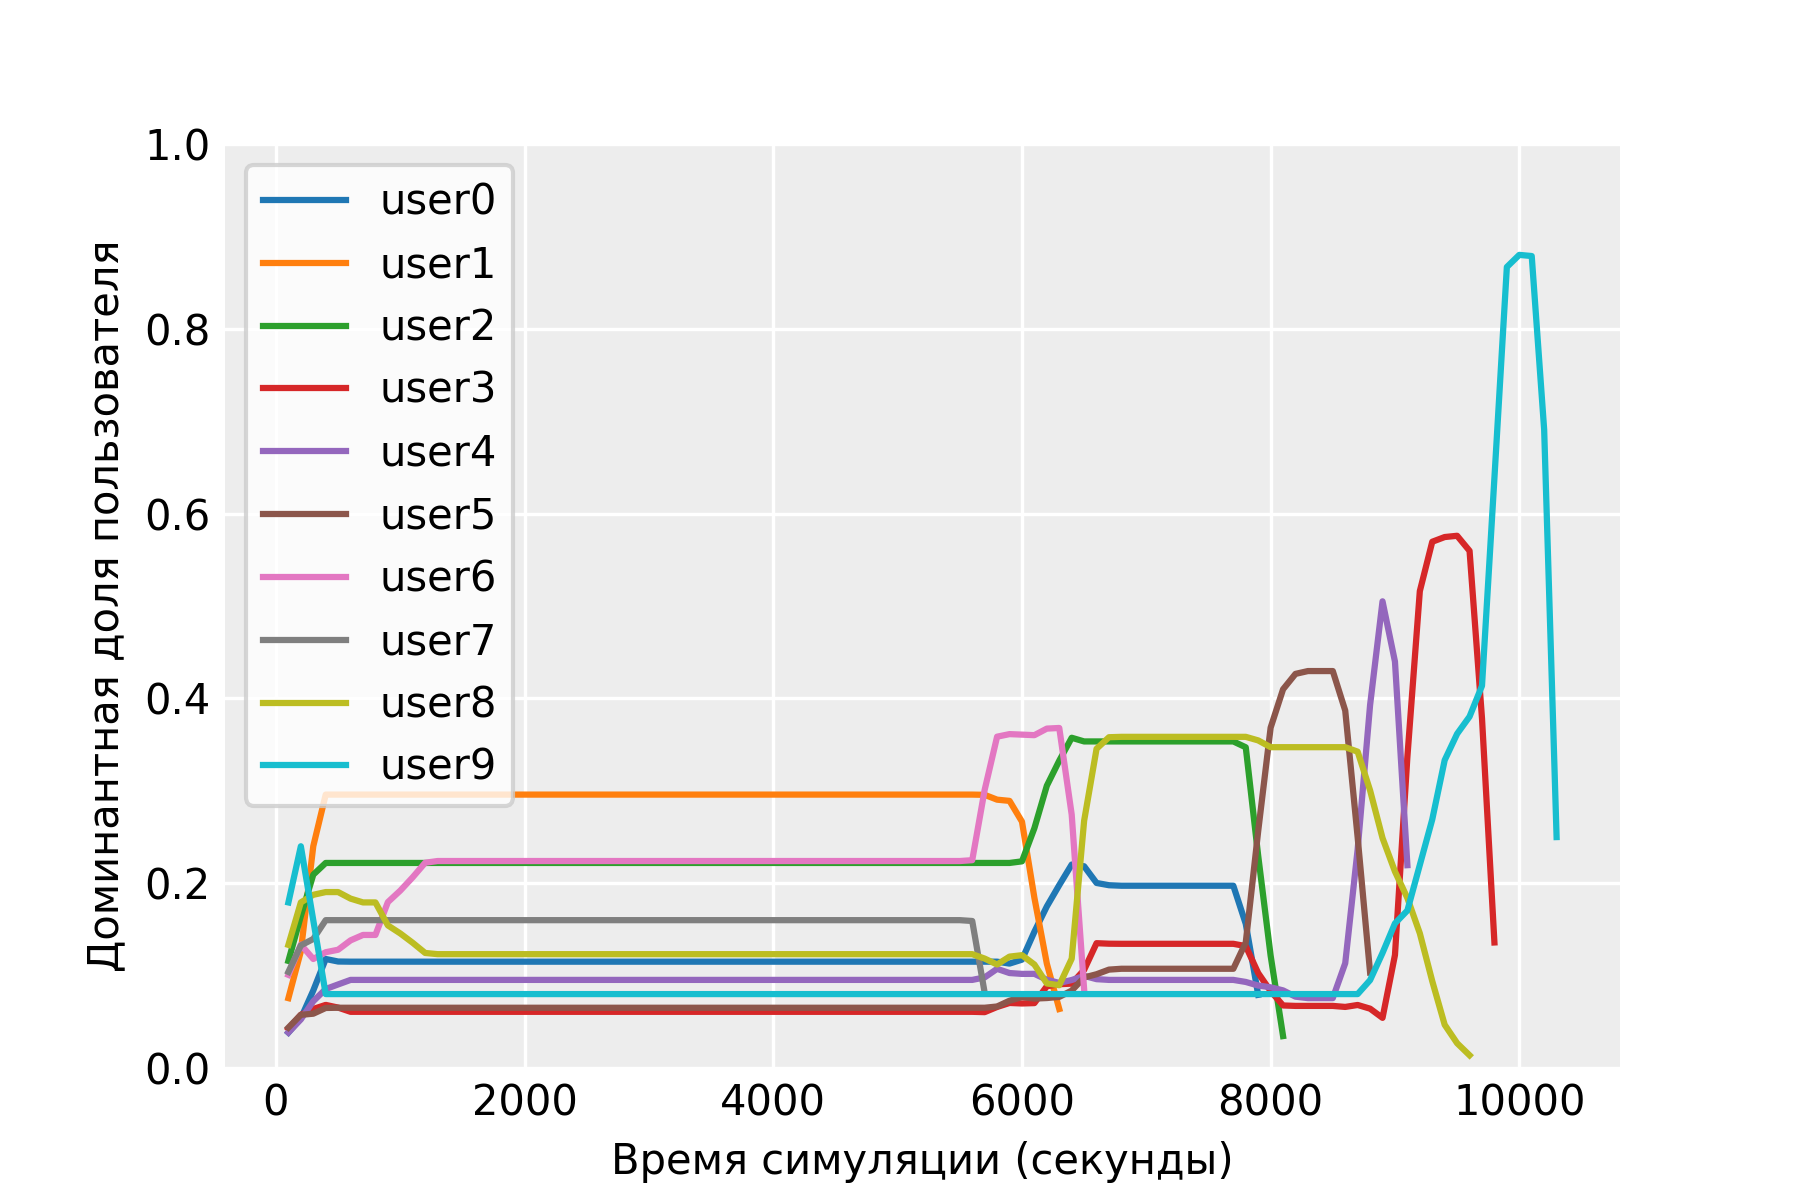
\includegraphics[width=\linewidth]{images/fair_share_0}
        \caption{$f = 0.0$}
        \label{fig:fair_share_0}
    \end{subfigure}
    \begin{subfigure}{0.49\linewidth}
        \centering
        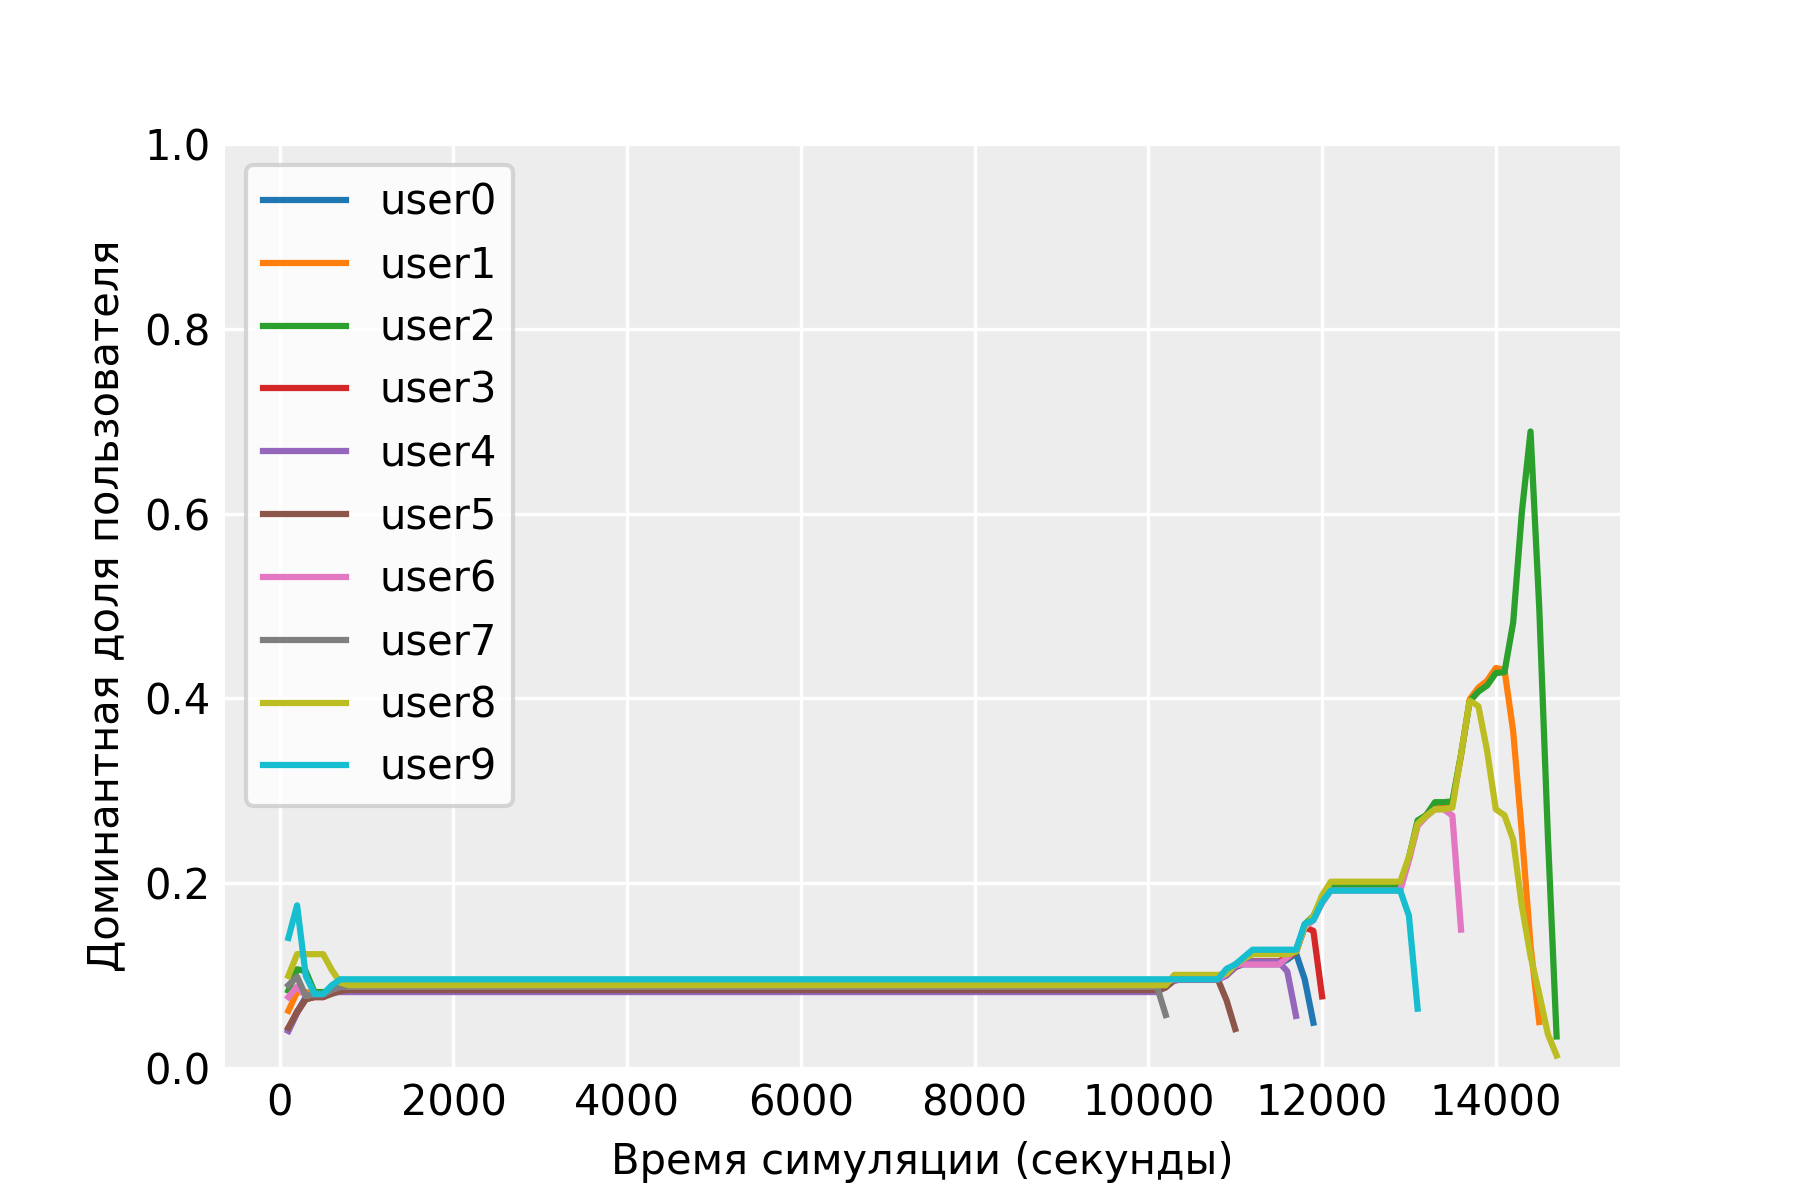
\includegraphics[width=\linewidth]{images/fair_share_1}
        \caption{$f = 1.0$}
        \label{fig:fair_share_1}
    \end{subfigure}

    \begin{subfigure}{0.49\linewidth}
        \centering
        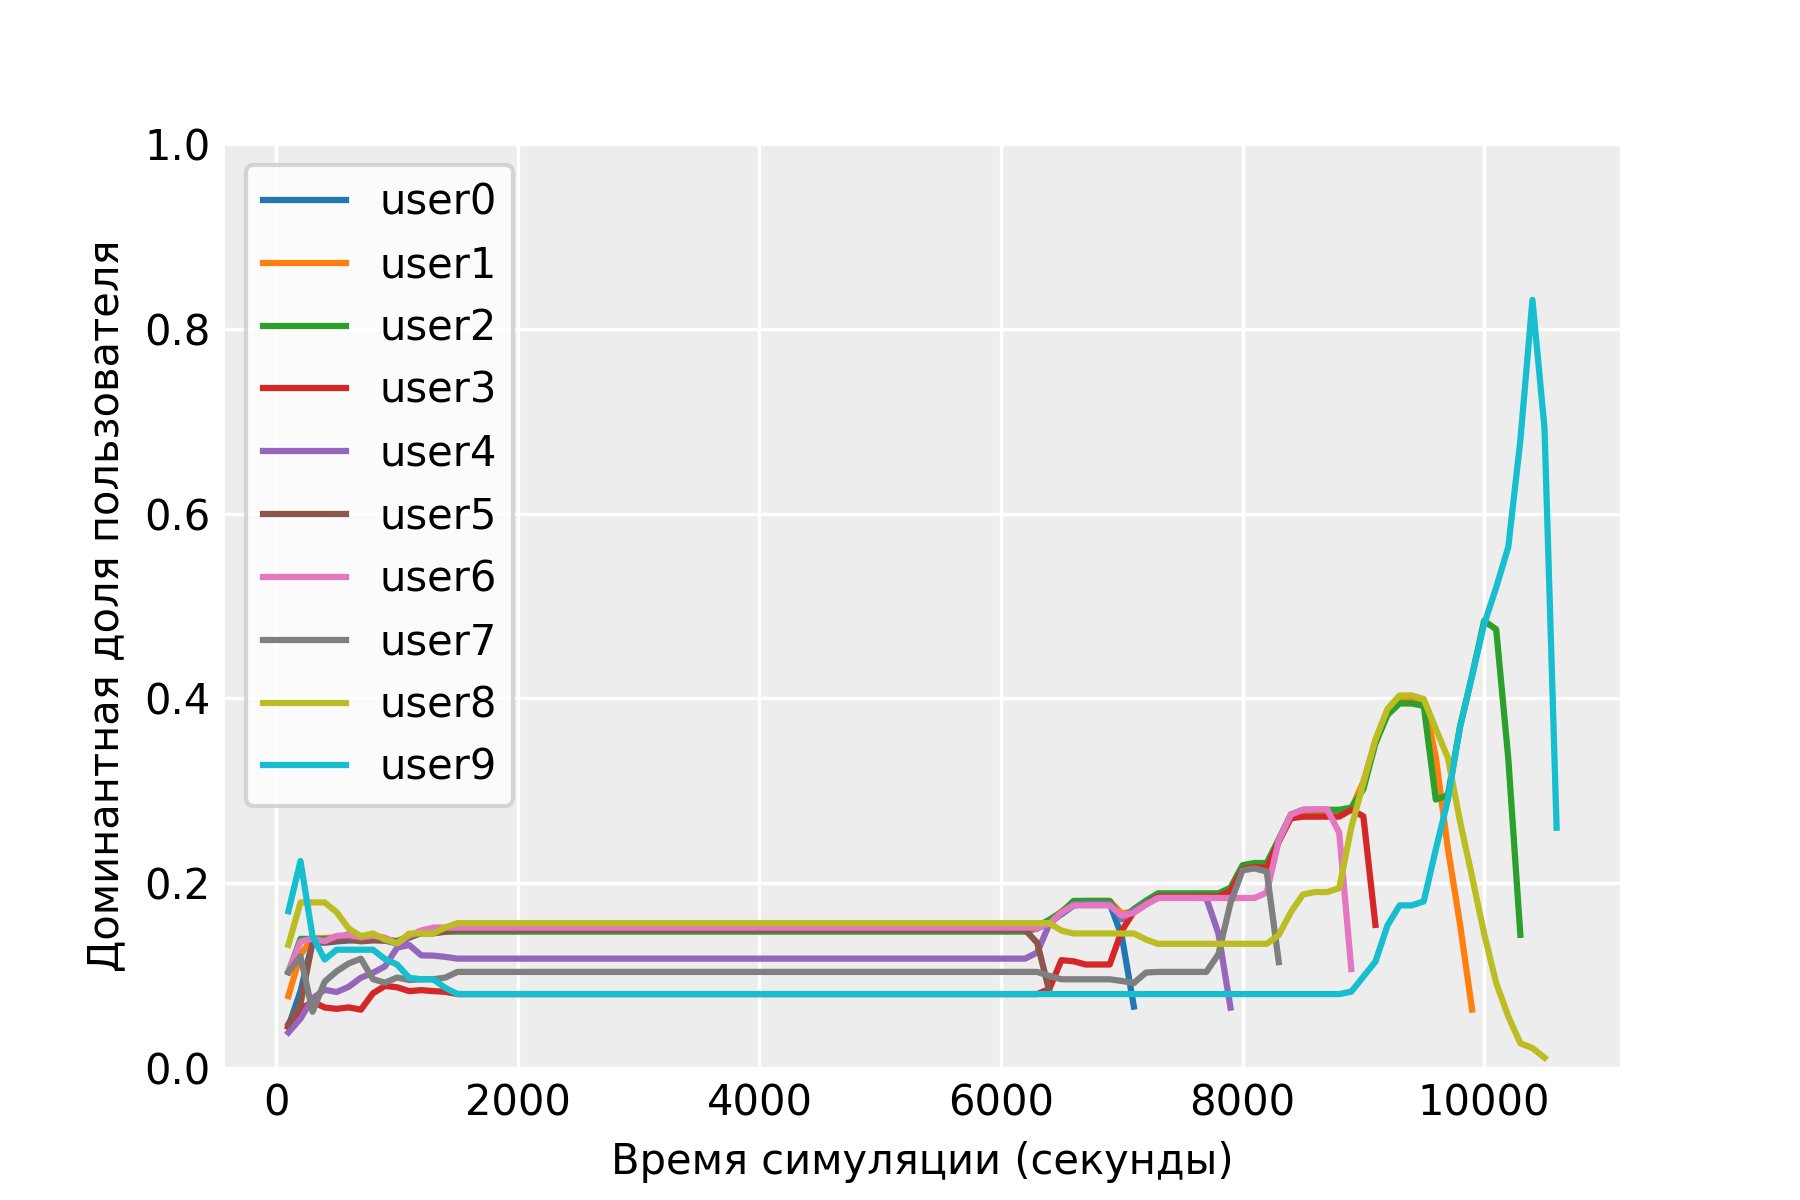
\includegraphics[width=\linewidth]{images/fair_share_05}
        \caption{$f = 0.5$}
        \label{fig:fair_share_05}
    \end{subfigure}
    \begin{subfigure}{0.49\linewidth}
        \centering
        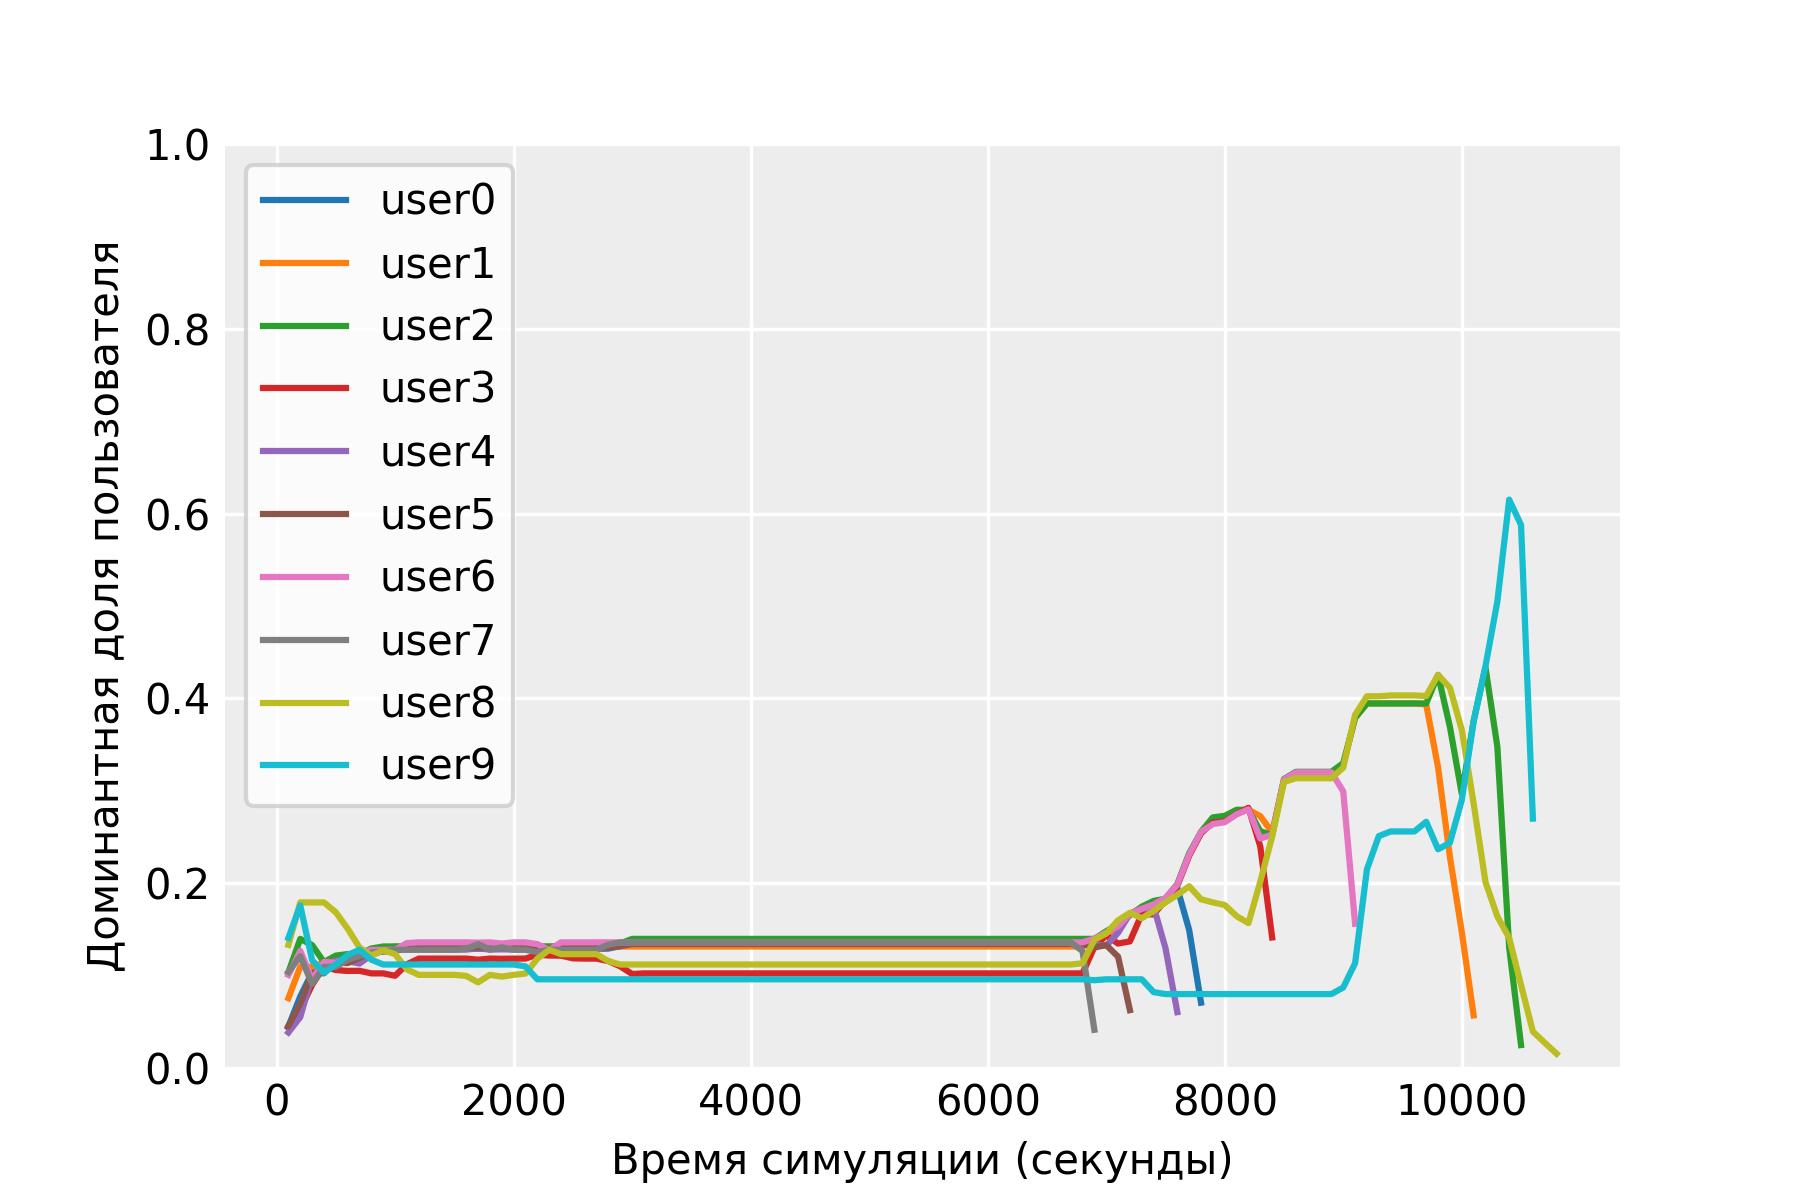
\includegraphics[width=\linewidth]{images/fair_share_06}
        \caption{$f = 0.6$}
        \label{fig:fair_share_06}
    \end{subfigure}
    \caption{Распределение доминантных долей использования кластера пользователями при различных коэффициентах справедливости $f$}
    \label{fig:fairness-results}
\end{figure}

Ожидаемо можно отметить, что при $f = 1$ доли у всех пользователей абсолютно одинаковые. В случае, когда у какого-то пользователя заканчиваются задачи, освободившиеся ресурсы равномерно распределяются по оставшимся пользователям. Но по времени симуляции, и по утилизации (графики \ref{fig:utilization-results}) видно, что это не самый лучший вариант занять кластер. А при $f = 0$ планировщик по сути сортирует пользователей по тому, насколько хорошо их задачи подходят под кластер.

Таким образом можно сделать вывод, что для такой конфигурации кластера и такой нагрузки оптимальный параметр справедливости для классического алгоритма \texttt{Tetris} будет $f = 0.6$. Именно с целью проверки подобных гипотез можно использовать симулятор вместо того, чтобы запускать все эти эксперименты на реальном кластере, т.к. для проведения подобного эксперимента в симуляторе потребуется всего несколько секунд. 

\subsection{Детерминированность симуляции}

Важным аспектом любой симуляции является воспроизводимость результатов. Фреймворк \texttt{DSLab} предоставляет универсальный интерфейс доступа к генератору случайных чисел в симуляции, который зависит только от переданного в симуляцию сида. Реализованный симулятор полностью использует эту возможность и является детерминированным при условии детерминированности алгоритма планирования. Очень важным является использование генератора случайных чисел из переданного в планировщик контекста (см. интерфейс \ref{fig:scheduler-interface}), однако в стандартных структурах данных языка \texttt{Rust} используется другой генератор случайных чисел, и это необходимо учитывать. Например, при итерации по ключам стандартной хэш-таблицы они будут возвращаться в разном порядке в зависимости от запуска программы. 

\section{Заключение}\label{sec:conclusion}

В рамках ВКР удалось реализовать многофункциональный и производительный симулятор вычислительного кластера. Код симулятора опубликован в открытом доступе на GitHub\cite{dslab-cluster-scheduling-repo}. В этом же репозитории представлены и примеры запуска симулятора в разных конфигурациях. Как результат работы можно выделить основное достижение: возможность пользователям исключительно гибко (по сравнению со всеми другими симуляциями) настраивать профиль загрузки сервера. Использование асинхронных примитивов языка \texttt{Rust} дает много возможностей для такого точного описания нагрузки. При этом, поддерживаются и более простые сценарии использования симулятора, в которых достигается высокая производительность.

C помощью симулятора проведены несколько экспериментов, которые показывают его применимость на больших симуляциях и в разных моделях планирования: справедливого распределения ресурсов между пользователями и  оптимальной упаковки задач на кластере. 


В качестве дальнейшего развития симулятора можно модифицировать модули \texttt{DSLab}, сделав возможной более полную отмену задач (добавить такой функционал в модулях \texttt{dslab-network} и \texttt{dslab-disk}). 


